% **************************************************************************************************************
% A Classic Thesis Style
% An Homage to The Elements of Typographic Style
%
% Copyright (C) 2015 André Miede http://www.miede.de
%
% If you like the style then I would appreciate a postcard. My address 
% can be found in the file ClassicThesis.pdf. A collection of the 
% postcards I received so far is available online at 
% http://postcards.miede.de
%
% License: This program is free software; you can redistribute it and/or
% modify it under the terms of the GNU General Public License as published
% by5. Utilizar o método de autômato celular com a melhor regra de transição
% para, the Free Software Foundation; either version 2 of the License, or (at
% your option) any later version.
%
% This program is distributed in the hope that it will be useful,
% but WITHOUT ANY WARRANTY; without even the implied warranty of
% MERCHANTABILITY or FITNESS FOR A PARTICULAR PURPOSE.  See the
% GNU General Public License for more details.
%
% You should have received a copy of the GNU General Public License
% along with this program; see the file COPYING.  If not, write to
% the Free Software Foundation, Inc., 59 Temple Place - Suite 330,
% Boston, MA 02111-1307, USA.
%
% **************************************************************************************************************
\RequirePackage{fix-cm} % fix some la\cite{Rose:2001}tex issues see: http://texdoc.net/texmf-dist/doc/latex/base/fixltx2e.pdf
\documentclass[ twoside,openright,titlepage,numbers=noenddot,headinclude,%1headlines,% letterpaper a4paper
                footinclude=true,cleardoublepage=empty,abstractoff, % <--- obsolete, remove (todo)
                BCOR=5mm,paper=a4,fontsize=11pt,%11pt,a4paper,%  ngerman,
                american,%
                ]{scrreprt}

%********************************************************************
% Note: Make all your adjustments in here
%*******************************************************
% ****************************************************************************************************
% classicthesis-config.tex 
% formerly known as loadpackages.sty, classicthesis-ldpkg.sty, and classicthesis-preamble.sty 
% Use it at the beginning of your ClassicThesis.tex, or as a LaTeX Preamble 
% in your ClassicThesis.{tex,lyx} with % ****************************************************************************************************
% classicthesis-config.tex 
% formerly known as loadpackages.sty, classicthesis-ldpkg.sty, and classicthesis-preamble.sty 
% Use it at the beginning of your ClassicThesis.tex, or as a LaTeX Preamble 
% in your ClassicThesis.{tex,lyx} with % ****************************************************************************************************
% classicthesis-config.tex 
% formerly known as loadpackages.sty, classicthesis-ldpkg.sty, and classicthesis-preamble.sty 
% Use it at the beginning of your ClassicThesis.tex, or as a LaTeX Preamble 
% in your ClassicThesis.{tex,lyx} with \input{classicthesis-config}
% ****************************************************************************************************  
% If you like the classicthesis, then I would appreciate a postcard. 
% My address can be found in the file ClassicThesis.pdf. A collection 
% of the postcards I received so far is available online at 
% http://postcards.miede.de
% ****************************************************************************************************


% ****************************************************************************************************
% 0. Set the encoding of your files.
% ****************************************************************************************************
\PassOptionsToPackage{latin2,latin9}{inputenc}
 \usepackage{inputenc}

% ****************************************************************************************************
% 1. Configure classicthesis for your needs here, e.g., remove "drafting" below 
% in order to deactivate the time-stamp on the pages
% ****************************************************************************************************
\PassOptionsToPackage{eulerchapternumbers,listings,drafting,%
					 pdfspacing,floatperchapter,%linedheaders,%
					 subfig,beramono,parts}{classicthesis}                                        
% ********************************************************************
% Available options for classicthesis.sty 
% (see ClassicThesis.pdf for more information):
% drafting
% parts nochapters linedheaders
% eulerchapternumbers beramono eulermath pdfspacing minionprospacing
% tocaligned dottedtoc manychapters
% listings floatperchapter subfig
% ********************************************************************

% ********************************************************************
% Triggers for this config
% ********************************************************************
\usepackage{ifthen}
\newboolean{enable-backrefs} % enable backrefs in the bibliography
\setboolean{enable-backrefs}{true} % true false
% ****************************************************************************************************


% ****************************************************************************************************
% 2. Personal data and user ad-hoc commands
% ****************************************************************************************************
\newcommand{\myTitle}{A Classic Thesis Style\xspace}
\newcommand{\mySubtitle}{An Homage to The Elements of Typographic Style\xspace}
\newcommand{\myDegree}{Doktor-Ingenieur (Dr.-Ing.)\xspace}
\newcommand{\myName}{Andr\'e Miede\xspace}
\newcommand{\myProf}{Put name here\xspace}
\newcommand{\myOtherProf}{Put name here\xspace}
\newcommand{\mySupervisor}{Put name here\xspace}
\newcommand{\myFaculty}{Put data here\xspace}
\newcommand{\myDepartment}{Put data here\xspace}
\newcommand{\myUni}{Put data here\xspace}
\newcommand{\myLocation}{Saarbr\"ucken\xspace}
\newcommand{\myTime}{September 2015\xspace}
\newcommand{\myVersion}{version 4.2\xspace}

% ********************************************************************
% Setup, finetuning, and useful commands
% ********************************************************************
\newcounter{dummy} % necessary for correct hyperlinks (to index, bib, etc.)
\newlength{\abcd} % for ab..z string length calculation
\providecommand{\mLyX}{L\kern-.1667em\lower.25em\hbox{Y}\kern-.125emX\@}
\newcommand{\ie}{i.\,e.}
\newcommand{\Ie}{I.\,e.}
\newcommand{\eg}{e.\,g.}
\newcommand{\Eg}{E.\,g.} 
% ****************************************************************************************************


% ****************************************************************************************************
% 3. Loading some handy packages
% ****************************************************************************************************
% ******************************************************************** 
% Packages with options that might require adjustments
% ******************************************************************** 
%\PassOptionsToPackage{ngerman,american}{babel}   % change this to your language(s)
% Spanish languages need extra options in order to work with this template
%\PassOptionsToPackage{spanish,es-lcroman}{babel}
	\usepackage{babel}

\PassOptionsToPackage{square,numbers}{natbib}
 \usepackage{natbib}

\PassOptionsToPackage{fleqn}{amsmath}       % math environments and more by the AMS 
    \usepackage{amsmath}

% ******************************************************************** 
% General useful packages
% ******************************************************************** 
\PassOptionsToPackage{T1}{fontenc} % T2A for cyrillics
    \usepackage{fontenc}     
\usepackage{textcomp} % fix warning with missing font shapes
\usepackage{scrhack} % fix warnings when using KOMA with listings package          
\usepackage{xspace} % to get the spacing after macros right  
\usepackage{mparhack} % get marginpar right
\usepackage{fixltx2e} % fixes some LaTeX stuff --> since 2015 in the LaTeX kernel (see below)
%\usepackage[latest]{latexrelease} % will be used once available in more distributions (ISSUE #107)
\PassOptionsToPackage{printonlyused,smaller}{acronym}
    \usepackage{acronym} % nice macros for handling all acronyms in the thesis
   %\renewcommand{\bflabel}[1]{{#1}\hfill} % fix the list of acronyms --> no longer working
   %\renewcommand*{\aclabelfont}[1]{\spacedlowsmallcaps{#1}}
    \renewcommand*{\acsfont}[1]{{\rmfamily\mdseries\small#1}} 
% ****************************************************************************************************


% ****************************************************************************************************
% 4. Setup floats: tables, (sub)figures, and captions
% ****************************************************************************************************
\usepackage{tabularx} % better tables
    \setlength{\extrarowheight}{3pt} % increase table row height
\newcommand{\tableheadline}[1]{\multicolumn{1}{c}{\spacedlowsmallcaps{#1}}}
\newcommand{\myfloatalign}{\centering} % to be used with each float for alignment
\usepackage{caption}
% Thanks to cgnieder and Claus Lahiri
% http://tex.stackexchange.com/questions/69349/spacedlowsmallcaps-in-caption-label
% [REMOVED DUE TO OTHER PROBLEMS, SEE ISSUE #82]    
%\DeclareCaptionLabelFormat{smallcaps}{\bothIfFirst{#1}{~}\MakeTextLowercase{\textsc{#2}}}
%\captionsetup{font=small,labelformat=smallcaps} % format=hang,
\captionsetup{font=small} % format=hang,
\usepackage{subfig}  
% ****************************************************************************************************


% ****************************************************************************************************
% 5. Setup code listings
% ****************************************************************************************************
\usepackage{listings} 
%\lstset{emph={trueIndex,root},emphstyle=\color{BlueViolet}}%\underbar} % for special keywords
\lstset{language=[LaTeX]Tex,%C++,
    keywordstyle=\color{RoyalBlue},%\bfseries,
    basicstyle=\small\ttfamily,
    %identifierstyle=\color{NavyBlue},
    commentstyle=\color{Green}\ttfamily,
    stringstyle=\rmfamily,
    numbers=none,%left,%
    numberstyle=\scriptsize,%\tiny
    stepnumber=5,
    numbersep=8pt,
    showstringspaces=false,
    breaklines=true,
    frameround=ftff,
    frame=single,
    belowcaptionskip=.75\baselineskip
    %frame=L
} 
% ****************************************************************************************************             


% ****************************************************************************************************
% 6. PDFLaTeX, hyperreferences and citation backreferences
% ****************************************************************************************************
% ********************************************************************
% Using PDFLaTeX
% ********************************************************************
\PassOptionsToPackage{pdftex,hyperfootnotes=false,pdfpagelabels}{hyperref}
    \usepackage{hyperref}  % backref linktocpage pagebackref
\pdfcompresslevel=9
\pdfadjustspacing=1 
\PassOptionsToPackage{pdftex}{graphicx}
    \usepackage{graphicx}
 
% ********************************************************************
% Setup the style of the backrefs from the bibliography
% (translate the options to any language you use)
% ********************************************************************
\newcommand{\backrefnotcitedstring}{\relax}%(Not cited.)
\newcommand{\backrefcitedsinglestring}[1]{(Cited on page~#1.)}
\newcommand{\backrefcitedmultistring}[1]{(Cited on pages~#1.)}
\ifthenelse{\boolean{enable-backrefs}}%
{%
		\PassOptionsToPackage{hyperpageref}{backref}
		\usepackage{backref} % to be loaded after hyperref package
		   \renewcommand{\backreftwosep}{ and~} % separate 2 pages
		   \renewcommand{\backreflastsep}{, and~} % separate last of longer list
		   \renewcommand*{\backref}[1]{}  % disable standard
		   \renewcommand*{\backrefalt}[4]{% detailed backref
		      \ifcase #1 %
		         \backrefnotcitedstring%
		      \or%
		         \backrefcitedsinglestring{#2}%
		      \else%
		         \backrefcitedmultistring{#2}%
		      \fi}%
}{\relax}

% ********************************************************************
% Hyperreferences
% ********************************************************************
\hypersetup{%
    %draft, % = no hyperlinking at all (useful in b/w printouts)
    colorlinks=true, linktocpage=true, pdfstartpage=3, pdfstartview=FitV,%
    % uncomment the following line if you want to have black links (e.g., for printing)
    %colorlinks=false, linktocpage=false, pdfstartpage=3, pdfstartview=FitV, pdfborder={0 0 0},%
    breaklinks=true, pdfpagemode=UseNone, pageanchor=true, pdfpagemode=UseOutlines,%
    plainpages=false, bookmarksnumbered, bookmarksopen=true, bookmarksopenlevel=1,%
    hypertexnames=true, pdfhighlight=/O,%nesting=true,%frenchlinks,%
    urlcolor=webbrown, linkcolor=RoyalBlue, citecolor=webgreen, %pagecolor=RoyalBlue,%
    %urlcolor=Black, linkcolor=Black, citecolor=Black, %pagecolor=Black,%
    pdftitle={\myTitle},%
    pdfauthor={\textcopyright\ \myName, \myUni, \myFaculty},%
    pdfsubject={},%
    pdfkeywords={},%
    pdfcreator={pdfLaTeX},%
    pdfproducer={LaTeX with hyperref and classicthesis}%
}   

% ********************************************************************
% Setup autoreferences
% ********************************************************************
% There are some issues regarding autorefnames
% http://www.ureader.de/msg/136221647.aspx
% http://www.tex.ac.uk/cgi-bin/texfaq2html?label=latexwords
% you have to redefine the makros for the 
% language you use, e.g., american, ngerman
% (as chosen when loading babel/AtBeginDocument)
% ********************************************************************
\makeatletter
\@ifpackageloaded{babel}%
    {%
       \addto\extrasamerican{%
			\renewcommand*{\figureautorefname}{Figure}%
			\renewcommand*{\tableautorefname}{Table}%
			\renewcommand*{\partautorefname}{Part}%
			\renewcommand*{\chapterautorefname}{Chapter}%
			\renewcommand*{\sectionautorefname}{Section}%
			\renewcommand*{\subsectionautorefname}{Section}%
			\renewcommand*{\subsubsectionautorefname}{Section}%     
                }%
       \addto\extrasngerman{% 
			\renewcommand*{\paragraphautorefname}{Absatz}%
			\renewcommand*{\subparagraphautorefname}{Unterabsatz}%
			\renewcommand*{\footnoteautorefname}{Fu\"snote}%
			\renewcommand*{\FancyVerbLineautorefname}{Zeile}%
			\renewcommand*{\theoremautorefname}{Theorem}%
			\renewcommand*{\appendixautorefname}{Anhang}%
			\renewcommand*{\equationautorefname}{Gleichung}%        
			\renewcommand*{\itemautorefname}{Punkt}%
                }%  
            % Fix to getting autorefs for subfigures right (thanks to Belinda Vogt for changing the definition)
            \providecommand{\subfigureautorefname}{\figureautorefname}%             
    }{\relax}
\makeatother


% ****************************************************************************************************
% 7. Last calls before the bar closes
% ****************************************************************************************************
% ********************************************************************
% Development Stuff
% ********************************************************************
\listfiles
%\PassOptionsToPackage{l2tabu,orthodox,abort}{nag}
%   \usepackage{nag}
%\PassOptionsToPackage{warning, all}{onlyamsmath}
%   \usepackage{onlyamsmath}

% ********************************************************************
% Last, but not least...
% ********************************************************************
\usepackage{classicthesis} 
% ****************************************************************************************************


% ****************************************************************************************************
% 8. Further adjustments (experimental)
% ****************************************************************************************************
% ********************************************************************
% Changing the text area
% ********************************************************************
%\linespread{1.05} % a bit more for Palatino
%\areaset[current]{312pt}{761pt} % 686 (factor 2.2) + 33 head + 42 head \the\footskip
%\setlength{\marginparwidth}{7em}%
%\setlength{\marginparsep}{2em}%

% ********************************************************************
% Using different fonts
% ********************************************************************
%\usepackage[oldstylenums]{kpfonts} % oldstyle notextcomp
%\usepackage[osf]{libertine}
%\usepackage[light,condensed,math]{iwona}
%\renewcommand{\sfdefault}{iwona}
%\usepackage{lmodern} % <-- no osf support :-(
%\usepackage{cfr-lm} % 
%\usepackage[urw-garamond]{mathdesign} <-- no osf support :-(
%\usepackage[default,osfigures]{opensans} % scale=0.95 
%\usepackage[sfdefault]{FiraSans}
% ****************************************************************************************************

% ****************************************************************************************************  
% If you like the classicthesis, then I would appreciate a postcard. 
% My address can be found in the file ClassicThesis.pdf. A collection 
% of the postcards I received so far is available online at 
% http://postcards.miede.de
% ****************************************************************************************************


% ****************************************************************************************************
% 0. Set the encoding of your files.
% ****************************************************************************************************
\PassOptionsToPackage{latin2,latin9}{inputenc}
 \usepackage{inputenc}

% ****************************************************************************************************
% 1. Configure classicthesis for your needs here, e.g., remove "drafting" below 
% in order to deactivate the time-stamp on the pages
% ****************************************************************************************************
\PassOptionsToPackage{eulerchapternumbers,listings,drafting,%
					 pdfspacing,floatperchapter,%linedheaders,%
					 subfig,beramono,parts}{classicthesis}                                        
% ********************************************************************
% Available options for classicthesis.sty 
% (see ClassicThesis.pdf for more information):
% drafting
% parts nochapters linedheaders
% eulerchapternumbers beramono eulermath pdfspacing minionprospacing
% tocaligned dottedtoc manychapters
% listings floatperchapter subfig
% ********************************************************************

% ********************************************************************
% Triggers for this config
% ********************************************************************
\usepackage{ifthen}
\newboolean{enable-backrefs} % enable backrefs in the bibliography
\setboolean{enable-backrefs}{true} % true false
% ****************************************************************************************************


% ****************************************************************************************************
% 2. Personal data and user ad-hoc commands
% ****************************************************************************************************
\newcommand{\myTitle}{A Classic Thesis Style\xspace}
\newcommand{\mySubtitle}{An Homage to The Elements of Typographic Style\xspace}
\newcommand{\myDegree}{Doktor-Ingenieur (Dr.-Ing.)\xspace}
\newcommand{\myName}{Andr\'e Miede\xspace}
\newcommand{\myProf}{Put name here\xspace}
\newcommand{\myOtherProf}{Put name here\xspace}
\newcommand{\mySupervisor}{Put name here\xspace}
\newcommand{\myFaculty}{Put data here\xspace}
\newcommand{\myDepartment}{Put data here\xspace}
\newcommand{\myUni}{Put data here\xspace}
\newcommand{\myLocation}{Saarbr\"ucken\xspace}
\newcommand{\myTime}{September 2015\xspace}
\newcommand{\myVersion}{version 4.2\xspace}

% ********************************************************************
% Setup, finetuning, and useful commands
% ********************************************************************
\newcounter{dummy} % necessary for correct hyperlinks (to index, bib, etc.)
\newlength{\abcd} % for ab..z string length calculation
\providecommand{\mLyX}{L\kern-.1667em\lower.25em\hbox{Y}\kern-.125emX\@}
\newcommand{\ie}{i.\,e.}
\newcommand{\Ie}{I.\,e.}
\newcommand{\eg}{e.\,g.}
\newcommand{\Eg}{E.\,g.} 
% ****************************************************************************************************


% ****************************************************************************************************
% 3. Loading some handy packages
% ****************************************************************************************************
% ******************************************************************** 
% Packages with options that might require adjustments
% ******************************************************************** 
%\PassOptionsToPackage{ngerman,american}{babel}   % change this to your language(s)
% Spanish languages need extra options in order to work with this template
%\PassOptionsToPackage{spanish,es-lcroman}{babel}
	\usepackage{babel}

\PassOptionsToPackage{square,numbers}{natbib}
 \usepackage{natbib}

\PassOptionsToPackage{fleqn}{amsmath}       % math environments and more by the AMS 
    \usepackage{amsmath}

% ******************************************************************** 
% General useful packages
% ******************************************************************** 
\PassOptionsToPackage{T1}{fontenc} % T2A for cyrillics
    \usepackage{fontenc}     
\usepackage{textcomp} % fix warning with missing font shapes
\usepackage{scrhack} % fix warnings when using KOMA with listings package          
\usepackage{xspace} % to get the spacing after macros right  
\usepackage{mparhack} % get marginpar right
\usepackage{fixltx2e} % fixes some LaTeX stuff --> since 2015 in the LaTeX kernel (see below)
%\usepackage[latest]{latexrelease} % will be used once available in more distributions (ISSUE #107)
\PassOptionsToPackage{printonlyused,smaller}{acronym}
    \usepackage{acronym} % nice macros for handling all acronyms in the thesis
   %\renewcommand{\bflabel}[1]{{#1}\hfill} % fix the list of acronyms --> no longer working
   %\renewcommand*{\aclabelfont}[1]{\spacedlowsmallcaps{#1}}
    \renewcommand*{\acsfont}[1]{{\rmfamily\mdseries\small#1}} 
% ****************************************************************************************************


% ****************************************************************************************************
% 4. Setup floats: tables, (sub)figures, and captions
% ****************************************************************************************************
\usepackage{tabularx} % better tables
    \setlength{\extrarowheight}{3pt} % increase table row height
\newcommand{\tableheadline}[1]{\multicolumn{1}{c}{\spacedlowsmallcaps{#1}}}
\newcommand{\myfloatalign}{\centering} % to be used with each float for alignment
\usepackage{caption}
% Thanks to cgnieder and Claus Lahiri
% http://tex.stackexchange.com/questions/69349/spacedlowsmallcaps-in-caption-label
% [REMOVED DUE TO OTHER PROBLEMS, SEE ISSUE #82]    
%\DeclareCaptionLabelFormat{smallcaps}{\bothIfFirst{#1}{~}\MakeTextLowercase{\textsc{#2}}}
%\captionsetup{font=small,labelformat=smallcaps} % format=hang,
\captionsetup{font=small} % format=hang,
\usepackage{subfig}  
% ****************************************************************************************************


% ****************************************************************************************************
% 5. Setup code listings
% ****************************************************************************************************
\usepackage{listings} 
%\lstset{emph={trueIndex,root},emphstyle=\color{BlueViolet}}%\underbar} % for special keywords
\lstset{language=[LaTeX]Tex,%C++,
    keywordstyle=\color{RoyalBlue},%\bfseries,
    basicstyle=\small\ttfamily,
    %identifierstyle=\color{NavyBlue},
    commentstyle=\color{Green}\ttfamily,
    stringstyle=\rmfamily,
    numbers=none,%left,%
    numberstyle=\scriptsize,%\tiny
    stepnumber=5,
    numbersep=8pt,
    showstringspaces=false,
    breaklines=true,
    frameround=ftff,
    frame=single,
    belowcaptionskip=.75\baselineskip
    %frame=L
} 
% ****************************************************************************************************             


% ****************************************************************************************************
% 6. PDFLaTeX, hyperreferences and citation backreferences
% ****************************************************************************************************
% ********************************************************************
% Using PDFLaTeX
% ********************************************************************
\PassOptionsToPackage{pdftex,hyperfootnotes=false,pdfpagelabels}{hyperref}
    \usepackage{hyperref}  % backref linktocpage pagebackref
\pdfcompresslevel=9
\pdfadjustspacing=1 
\PassOptionsToPackage{pdftex}{graphicx}
    \usepackage{graphicx}
 
% ********************************************************************
% Setup the style of the backrefs from the bibliography
% (translate the options to any language you use)
% ********************************************************************
\newcommand{\backrefnotcitedstring}{\relax}%(Not cited.)
\newcommand{\backrefcitedsinglestring}[1]{(Cited on page~#1.)}
\newcommand{\backrefcitedmultistring}[1]{(Cited on pages~#1.)}
\ifthenelse{\boolean{enable-backrefs}}%
{%
		\PassOptionsToPackage{hyperpageref}{backref}
		\usepackage{backref} % to be loaded after hyperref package
		   \renewcommand{\backreftwosep}{ and~} % separate 2 pages
		   \renewcommand{\backreflastsep}{, and~} % separate last of longer list
		   \renewcommand*{\backref}[1]{}  % disable standard
		   \renewcommand*{\backrefalt}[4]{% detailed backref
		      \ifcase #1 %
		         \backrefnotcitedstring%
		      \or%
		         \backrefcitedsinglestring{#2}%
		      \else%
		         \backrefcitedmultistring{#2}%
		      \fi}%
}{\relax}

% ********************************************************************
% Hyperreferences
% ********************************************************************
\hypersetup{%
    %draft, % = no hyperlinking at all (useful in b/w printouts)
    colorlinks=true, linktocpage=true, pdfstartpage=3, pdfstartview=FitV,%
    % uncomment the following line if you want to have black links (e.g., for printing)
    %colorlinks=false, linktocpage=false, pdfstartpage=3, pdfstartview=FitV, pdfborder={0 0 0},%
    breaklinks=true, pdfpagemode=UseNone, pageanchor=true, pdfpagemode=UseOutlines,%
    plainpages=false, bookmarksnumbered, bookmarksopen=true, bookmarksopenlevel=1,%
    hypertexnames=true, pdfhighlight=/O,%nesting=true,%frenchlinks,%
    urlcolor=webbrown, linkcolor=RoyalBlue, citecolor=webgreen, %pagecolor=RoyalBlue,%
    %urlcolor=Black, linkcolor=Black, citecolor=Black, %pagecolor=Black,%
    pdftitle={\myTitle},%
    pdfauthor={\textcopyright\ \myName, \myUni, \myFaculty},%
    pdfsubject={},%
    pdfkeywords={},%
    pdfcreator={pdfLaTeX},%
    pdfproducer={LaTeX with hyperref and classicthesis}%
}   

% ********************************************************************
% Setup autoreferences
% ********************************************************************
% There are some issues regarding autorefnames
% http://www.ureader.de/msg/136221647.aspx
% http://www.tex.ac.uk/cgi-bin/texfaq2html?label=latexwords
% you have to redefine the makros for the 
% language you use, e.g., american, ngerman
% (as chosen when loading babel/AtBeginDocument)
% ********************************************************************
\makeatletter
\@ifpackageloaded{babel}%
    {%
       \addto\extrasamerican{%
			\renewcommand*{\figureautorefname}{Figure}%
			\renewcommand*{\tableautorefname}{Table}%
			\renewcommand*{\partautorefname}{Part}%
			\renewcommand*{\chapterautorefname}{Chapter}%
			\renewcommand*{\sectionautorefname}{Section}%
			\renewcommand*{\subsectionautorefname}{Section}%
			\renewcommand*{\subsubsectionautorefname}{Section}%     
                }%
       \addto\extrasngerman{% 
			\renewcommand*{\paragraphautorefname}{Absatz}%
			\renewcommand*{\subparagraphautorefname}{Unterabsatz}%
			\renewcommand*{\footnoteautorefname}{Fu\"snote}%
			\renewcommand*{\FancyVerbLineautorefname}{Zeile}%
			\renewcommand*{\theoremautorefname}{Theorem}%
			\renewcommand*{\appendixautorefname}{Anhang}%
			\renewcommand*{\equationautorefname}{Gleichung}%        
			\renewcommand*{\itemautorefname}{Punkt}%
                }%  
            % Fix to getting autorefs for subfigures right (thanks to Belinda Vogt for changing the definition)
            \providecommand{\subfigureautorefname}{\figureautorefname}%             
    }{\relax}
\makeatother


% ****************************************************************************************************
% 7. Last calls before the bar closes
% ****************************************************************************************************
% ********************************************************************
% Development Stuff
% ********************************************************************
\listfiles
%\PassOptionsToPackage{l2tabu,orthodox,abort}{nag}
%   \usepackage{nag}
%\PassOptionsToPackage{warning, all}{onlyamsmath}
%   \usepackage{onlyamsmath}

% ********************************************************************
% Last, but not least...
% ********************************************************************
\usepackage{classicthesis} 
% ****************************************************************************************************


% ****************************************************************************************************
% 8. Further adjustments (experimental)
% ****************************************************************************************************
% ********************************************************************
% Changing the text area
% ********************************************************************
%\linespread{1.05} % a bit more for Palatino
%\areaset[current]{312pt}{761pt} % 686 (factor 2.2) + 33 head + 42 head \the\footskip
%\setlength{\marginparwidth}{7em}%
%\setlength{\marginparsep}{2em}%

% ********************************************************************
% Using different fonts
% ********************************************************************
%\usepackage[oldstylenums]{kpfonts} % oldstyle notextcomp
%\usepackage[osf]{libertine}
%\usepackage[light,condensed,math]{iwona}
%\renewcommand{\sfdefault}{iwona}
%\usepackage{lmodern} % <-- no osf support :-(
%\usepackage{cfr-lm} % 
%\usepackage[urw-garamond]{mathdesign} <-- no osf support :-(
%\usepackage[default,osfigures]{opensans} % scale=0.95 
%\usepackage[sfdefault]{FiraSans}
% ****************************************************************************************************

% ****************************************************************************************************  
% If you like the classicthesis, then I would appreciate a postcard. 
% My address can be found in the file ClassicThesis.pdf. A collection 
% of the postcards I received so far is available online at 
% http://postcards.miede.de
% ****************************************************************************************************


% ****************************************************************************************************
% 0. Set the encoding of your files.
% ****************************************************************************************************
\PassOptionsToPackage{latin2,latin9}{inputenc}
 \usepackage{inputenc}

% ****************************************************************************************************
% 1. Configure classicthesis for your needs here, e.g., remove "drafting" below 
% in order to deactivate the time-stamp on the pages
% ****************************************************************************************************
\PassOptionsToPackage{eulerchapternumbers,listings,drafting,%
					 pdfspacing,floatperchapter,%linedheaders,%
					 subfig,beramono,parts}{classicthesis}                                        
% ********************************************************************
% Available options for classicthesis.sty 
% (see ClassicThesis.pdf for more information):
% drafting
% parts nochapters linedheaders
% eulerchapternumbers beramono eulermath pdfspacing minionprospacing
% tocaligned dottedtoc manychapters
% listings floatperchapter subfig
% ********************************************************************

% ********************************************************************
% Triggers for this config
% ********************************************************************
\usepackage{ifthen}
\newboolean{enable-backrefs} % enable backrefs in the bibliography
\setboolean{enable-backrefs}{true} % true false
% ****************************************************************************************************


% ****************************************************************************************************
% 2. Personal data and user ad-hoc commands
% ****************************************************************************************************
\newcommand{\myTitle}{A Classic Thesis Style\xspace}
\newcommand{\mySubtitle}{An Homage to The Elements of Typographic Style\xspace}
\newcommand{\myDegree}{Doktor-Ingenieur (Dr.-Ing.)\xspace}
\newcommand{\myName}{Andr\'e Miede\xspace}
\newcommand{\myProf}{Put name here\xspace}
\newcommand{\myOtherProf}{Put name here\xspace}
\newcommand{\mySupervisor}{Put name here\xspace}
\newcommand{\myFaculty}{Put data here\xspace}
\newcommand{\myDepartment}{Put data here\xspace}
\newcommand{\myUni}{Put data here\xspace}
\newcommand{\myLocation}{Saarbr\"ucken\xspace}
\newcommand{\myTime}{September 2015\xspace}
\newcommand{\myVersion}{version 4.2\xspace}

% ********************************************************************
% Setup, finetuning, and useful commands
% ********************************************************************
\newcounter{dummy} % necessary for correct hyperlinks (to index, bib, etc.)
\newlength{\abcd} % for ab..z string length calculation
\providecommand{\mLyX}{L\kern-.1667em\lower.25em\hbox{Y}\kern-.125emX\@}
\newcommand{\ie}{i.\,e.}
\newcommand{\Ie}{I.\,e.}
\newcommand{\eg}{e.\,g.}
\newcommand{\Eg}{E.\,g.} 
% ****************************************************************************************************


% ****************************************************************************************************
% 3. Loading some handy packages
% ****************************************************************************************************
% ******************************************************************** 
% Packages with options that might require adjustments
% ******************************************************************** 
%\PassOptionsToPackage{ngerman,american}{babel}   % change this to your language(s)
% Spanish languages need extra options in order to work with this template
%\PassOptionsToPackage{spanish,es-lcroman}{babel}
	\usepackage{babel}

\PassOptionsToPackage{square,numbers}{natbib}
 \usepackage{natbib}

\PassOptionsToPackage{fleqn}{amsmath}       % math environments and more by the AMS 
    \usepackage{amsmath}

% ******************************************************************** 
% General useful packages
% ******************************************************************** 
\PassOptionsToPackage{T1}{fontenc} % T2A for cyrillics
    \usepackage{fontenc}     
\usepackage{textcomp} % fix warning with missing font shapes
\usepackage{scrhack} % fix warnings when using KOMA with listings package          
\usepackage{xspace} % to get the spacing after macros right  
\usepackage{mparhack} % get marginpar right
\usepackage{fixltx2e} % fixes some LaTeX stuff --> since 2015 in the LaTeX kernel (see below)
%\usepackage[latest]{latexrelease} % will be used once available in more distributions (ISSUE #107)
\PassOptionsToPackage{printonlyused,smaller}{acronym}
    \usepackage{acronym} % nice macros for handling all acronyms in the thesis
   %\renewcommand{\bflabel}[1]{{#1}\hfill} % fix the list of acronyms --> no longer working
   %\renewcommand*{\aclabelfont}[1]{\spacedlowsmallcaps{#1}}
    \renewcommand*{\acsfont}[1]{{\rmfamily\mdseries\small#1}} 
% ****************************************************************************************************


% ****************************************************************************************************
% 4. Setup floats: tables, (sub)figures, and captions
% ****************************************************************************************************
\usepackage{tabularx} % better tables
    \setlength{\extrarowheight}{3pt} % increase table row height
\newcommand{\tableheadline}[1]{\multicolumn{1}{c}{\spacedlowsmallcaps{#1}}}
\newcommand{\myfloatalign}{\centering} % to be used with each float for alignment
\usepackage{caption}
% Thanks to cgnieder and Claus Lahiri
% http://tex.stackexchange.com/questions/69349/spacedlowsmallcaps-in-caption-label
% [REMOVED DUE TO OTHER PROBLEMS, SEE ISSUE #82]    
%\DeclareCaptionLabelFormat{smallcaps}{\bothIfFirst{#1}{~}\MakeTextLowercase{\textsc{#2}}}
%\captionsetup{font=small,labelformat=smallcaps} % format=hang,
\captionsetup{font=small} % format=hang,
\usepackage{subfig}  
% ****************************************************************************************************


% ****************************************************************************************************
% 5. Setup code listings
% ****************************************************************************************************
\usepackage{listings} 
%\lstset{emph={trueIndex,root},emphstyle=\color{BlueViolet}}%\underbar} % for special keywords
\lstset{language=[LaTeX]Tex,%C++,
    keywordstyle=\color{RoyalBlue},%\bfseries,
    basicstyle=\small\ttfamily,
    %identifierstyle=\color{NavyBlue},
    commentstyle=\color{Green}\ttfamily,
    stringstyle=\rmfamily,
    numbers=none,%left,%
    numberstyle=\scriptsize,%\tiny
    stepnumber=5,
    numbersep=8pt,
    showstringspaces=false,
    breaklines=true,
    frameround=ftff,
    frame=single,
    belowcaptionskip=.75\baselineskip
    %frame=L
} 
% ****************************************************************************************************             


% ****************************************************************************************************
% 6. PDFLaTeX, hyperreferences and citation backreferences
% ****************************************************************************************************
% ********************************************************************
% Using PDFLaTeX
% ********************************************************************
\PassOptionsToPackage{pdftex,hyperfootnotes=false,pdfpagelabels}{hyperref}
    \usepackage{hyperref}  % backref linktocpage pagebackref
\pdfcompresslevel=9
\pdfadjustspacing=1 
\PassOptionsToPackage{pdftex}{graphicx}
    \usepackage{graphicx}
 
% ********************************************************************
% Setup the style of the backrefs from the bibliography
% (translate the options to any language you use)
% ********************************************************************
\newcommand{\backrefnotcitedstring}{\relax}%(Not cited.)
\newcommand{\backrefcitedsinglestring}[1]{(Cited on page~#1.)}
\newcommand{\backrefcitedmultistring}[1]{(Cited on pages~#1.)}
\ifthenelse{\boolean{enable-backrefs}}%
{%
		\PassOptionsToPackage{hyperpageref}{backref}
		\usepackage{backref} % to be loaded after hyperref package
		   \renewcommand{\backreftwosep}{ and~} % separate 2 pages
		   \renewcommand{\backreflastsep}{, and~} % separate last of longer list
		   \renewcommand*{\backref}[1]{}  % disable standard
		   \renewcommand*{\backrefalt}[4]{% detailed backref
		      \ifcase #1 %
		         \backrefnotcitedstring%
		      \or%
		         \backrefcitedsinglestring{#2}%
		      \else%
		         \backrefcitedmultistring{#2}%
		      \fi}%
}{\relax}

% ********************************************************************
% Hyperreferences
% ********************************************************************
\hypersetup{%
    %draft, % = no hyperlinking at all (useful in b/w printouts)
    colorlinks=true, linktocpage=true, pdfstartpage=3, pdfstartview=FitV,%
    % uncomment the following line if you want to have black links (e.g., for printing)
    %colorlinks=false, linktocpage=false, pdfstartpage=3, pdfstartview=FitV, pdfborder={0 0 0},%
    breaklinks=true, pdfpagemode=UseNone, pageanchor=true, pdfpagemode=UseOutlines,%
    plainpages=false, bookmarksnumbered, bookmarksopen=true, bookmarksopenlevel=1,%
    hypertexnames=true, pdfhighlight=/O,%nesting=true,%frenchlinks,%
    urlcolor=webbrown, linkcolor=RoyalBlue, citecolor=webgreen, %pagecolor=RoyalBlue,%
    %urlcolor=Black, linkcolor=Black, citecolor=Black, %pagecolor=Black,%
    pdftitle={\myTitle},%
    pdfauthor={\textcopyright\ \myName, \myUni, \myFaculty},%
    pdfsubject={},%
    pdfkeywords={},%
    pdfcreator={pdfLaTeX},%
    pdfproducer={LaTeX with hyperref and classicthesis}%
}   

% ********************************************************************
% Setup autoreferences
% ********************************************************************
% There are some issues regarding autorefnames
% http://www.ureader.de/msg/136221647.aspx
% http://www.tex.ac.uk/cgi-bin/texfaq2html?label=latexwords
% you have to redefine the makros for the 
% language you use, e.g., american, ngerman
% (as chosen when loading babel/AtBeginDocument)
% ********************************************************************
\makeatletter
\@ifpackageloaded{babel}%
    {%
       \addto\extrasamerican{%
			\renewcommand*{\figureautorefname}{Figure}%
			\renewcommand*{\tableautorefname}{Table}%
			\renewcommand*{\partautorefname}{Part}%
			\renewcommand*{\chapterautorefname}{Chapter}%
			\renewcommand*{\sectionautorefname}{Section}%
			\renewcommand*{\subsectionautorefname}{Section}%
			\renewcommand*{\subsubsectionautorefname}{Section}%     
                }%
       \addto\extrasngerman{% 
			\renewcommand*{\paragraphautorefname}{Absatz}%
			\renewcommand*{\subparagraphautorefname}{Unterabsatz}%
			\renewcommand*{\footnoteautorefname}{Fu\"snote}%
			\renewcommand*{\FancyVerbLineautorefname}{Zeile}%
			\renewcommand*{\theoremautorefname}{Theorem}%
			\renewcommand*{\appendixautorefname}{Anhang}%
			\renewcommand*{\equationautorefname}{Gleichung}%        
			\renewcommand*{\itemautorefname}{Punkt}%
                }%  
            % Fix to getting autorefs for subfigures right (thanks to Belinda Vogt for changing the definition)
            \providecommand{\subfigureautorefname}{\figureautorefname}%             
    }{\relax}
\makeatother


% ****************************************************************************************************
% 7. Last calls before the bar closes
% ****************************************************************************************************
% ********************************************************************
% Development Stuff
% ********************************************************************
\listfiles
%\PassOptionsToPackage{l2tabu,orthodox,abort}{nag}
%   \usepackage{nag}
%\PassOptionsToPackage{warning, all}{onlyamsmath}
%   \usepackage{onlyamsmath}

% ********************************************************************
% Last, but not least...
% ********************************************************************
\usepackage{classicthesis} 
% ****************************************************************************************************


% ****************************************************************************************************
% 8. Further adjustments (experimental)
% ****************************************************************************************************
% ********************************************************************
% Changing the text area
% ********************************************************************
%\linespread{1.05} % a bit more for Palatino
%\areaset[current]{312pt}{761pt} % 686 (factor 2.2) + 33 head + 42 head \the\footskip
%\setlength{\marginparwidth}{7em}%
%\setlength{\marginparsep}{2em}%

% ********************************************************************
% Using different fonts
% ********************************************************************
%\usepackage[oldstylenums]{kpfonts} % oldstyle notextcomp
%\usepackage[osf]{libertine}
%\usepackage[light,condensed,math]{iwona}
%\renewcommand{\sfdefault}{iwona}
%\usepackage{lmodern} % <-- no osf support :-(
%\usepackage{cfr-lm} % 
%\usepackage[urw-garamond]{mathdesign} <-- no osf support :-(
%\usepackage[default,osfigures]{opensans} % scale=0.95 
%\usepackage[sfdefault]{FiraSans}
% ****************************************************************************************************


%********************************************************************
% Bibliographies
%*******************************************************
\addbibresource{bibliografia.bib}
\addbibresource[label=ownpubs]{AMiede_Publications.bib}

%********************************************************************
% Hyphenation
%*******************************************************
%\hyphenation{put special hyphenation here}

% ******************************************************************** %GO!GO!GO! MOVE IT! %*******************************************************
\begin{document} \frenchspacing \raggedbottom \selectlanguage{brazil} % american ngerman %\renewcommand*{\bibname}{new name} %\setbibpreamble{}
\pagenumbering{roman} \pagestyle{plain}
%******************************************************************** %Frontmatter %*******************************************************
%*******************************************************
% Little Dirty Titlepage
%*******************************************************
\thispagestyle{empty}
%\pdfbookmark[1]{Titel}{title}
%*******************************************************
\begin{center}
    \spacedlowsmallcaps{\myName} \\ \medskip                        

    \begingroup
        \color{Maroon}\spacedallcaps{\myTitle}
    \endgroup
\end{center}        
 %*******************************************************
% Titlepage
%*******************************************************
\begin{titlepage}
    % if you want the titlepage to be centered, uncomment and fine-tune the line below (KOMA classes environment)
    \begin{addmargin}[-1cm]{-3cm}
    \begin{center}
        \large  

        \hfill

        \vfill

        \begingroup
            \color{Maroon}\spacedallcaps{\myTitle} \\ \bigskip
        \endgroup

        \spacedlowsmallcaps{\myName}

        \vfill

        
\includegraphics[width=6cm]{gfx/TFZsuperellipse_bw} \\ \medskip

        \mySubtitle \\ \medskip   
        %\myDegree \\
        %\myDepartment \\                            
        %\myFaculty \\
        %\myUni \\ \bigskip

        \myTime\ -- \myVersion

        \vfill                      

    \end{center}  
  \end{addmargin}       
\end{titlepage}   
\thispagestyle{empty}

\hfill

\vfill

\noindent\myName: \textit{\myTitle,} \mySubtitle, %\myDegree, 
\textcopyright\ \myTime

%\bigskip
%
%\noindent\spacedlowsmallcaps{Supervisors}: \\
%\myProf \\
%\myOtherProf \\ 
%\mySupervisor
%
%\medskip
%
%\noindent\spacedlowsmallcaps{Location}: \\
%\myLocation
%
%\medskip
%
%\noindent\spacedlowsmallcaps{Time Frame}: \\
%\myTime
 
%\cleardoublepage%*******************************************************
% Dedication
%*******************************************************
\thispagestyle{empty}
%\phantomsection 
\refstepcounter{dummy}
\pdfbookmark[1]{Dedication}{Dedication}

\vspace*{3cm}

\begin{center}
    \emph{Ohana} means family. \\
    Family means nobody gets left behind, or forgotten. \\ \medskip
    --- Lilo \& Stitch    
\end{center}

\medskip

\begin{center}
    Dedicated to the loving memory of Rudolf Miede. \\ \smallskip
    1939\,--\,2005
\end{center}
%\cleardoublepage\include{FrontBackmatter/Foreword}
\cleardoublepage%*******************************************************
% Abstract
%*******************************************************
%\renewcommand{\abstractname}{Abstract}
\pdfbookmark[1]{Resumo}{Resumo}
\begingroup
\let\clearpage\relax
\let\cleardoublepage\relax
\let\cleardoublepage\relax

\chapter*{Resumo}
Short summary of the contents in English\dots a great guide by 
Kent Beck how to write good abstracts can be found here:  
\begin{center}
\url{https://plg.uwaterloo.ca/~migod/research/beckOOPSLA.html}
\end{center}

\vfill

\begin{otherlanguage}{american}
\pdfbookmark[1]{Abstract}{Abstract}
\chapter*{Abstract}
Resumo
\end{otherlanguage}

\endgroup			

\vfill 
%\cleardoublepage%*******************************************************
% Publications
%*******************************************************
\pdfbookmark[1]{Publications}{publications}
\chapter*{Publications}\graffito{This is just an early --~and currently ugly~-- test!}
This might come in handy for PhD theses: some ideas and figures have appeared previously in the following publications:

%\noindent Put your publications from the thesis here. The packages \texttt{multibib} or \texttt{bibtopic} etc. can be used to handle multiple different bibliographies in your document.

\begin{refsection}[ownpubs]
    \small
    \nocite{*} % is local to to the enclosing refsection
    \printbibliography[heading=none]
\end{refsection}

\emph{Attention}: This requires a separate run of \texttt{bibtex} for your \texttt{refsection}, \eg, \texttt{ClassicThesis1-blx} for this file. You might also use \texttt{biber} as the backend for \texttt{biblatex}. See also \url{http://tex.stackexchange.com/questions/128196/problem-with-refsection}. 
%\cleardoublepage%*******************************************************
% Acknowledgments
%*******************************************************
\pdfbookmark[1]{Acknowledgments}{acknowledgments}

\begin{flushright}{\slshape    
    We have seen that computer programming is an art, \\ 
    because it applies accumulated knowledge to the world, \\ 
    because it requires skill and ingenuity, and especially \\
    because it produces objects of beauty.} \\ \medskip
    --- \defcitealias{knuth:1974}{Donald E. Knuth}\citetalias{knuth:1974} \citep{knuth:1974}
\end{flushright}



\bigskip

\begingroup
\let\clearpage\relax
\let\cleardoublepage\relax
\let\cleardoublepage\relax
\chapter*{Acknowledgments}
Put your acknowledgments here.

Many thanks to everybody who already sent me a postcard!

Regarding the typography and other help, many thanks go to Marco 
Kuhlmann, Philipp Lehman, Lothar Schlesier, Jim Young, Lorenzo 
Pantieri and Enrico Gregorio\footnote{Members of GuIT (Gruppo 
Italiano Utilizzatori di \TeX\ e \LaTeX )}, J\"org Sommer, 
Joachim K\"ostler, Daniel Gottschlag, Denis Aydin, Paride 
Legovini, Steffen Prochnow, Nicolas Repp, Hinrich Harms, 
 Roland Winkler, Jörg Weber, Henri Menke, Claus Lahiri, 
 Clemens Niederberger, Stefano Bragaglia, Jörn Hees, 
 and the whole \LaTeX-community for support, ideas and 
 some great software.

\bigskip

\noindent\emph{Regarding \mLyX}: The \mLyX\ port was intially done by 
\emph{Nicholas Mariette} in March 2009 and continued by 
\emph{Ivo Pletikosi\'c} in 2011. Thank you very much for your 
work and for the contributions to the original style.


\endgroup




\pagestyle{scrheadings} \cleardoublepage%*******************************************************
% Table of Contents
%*******************************************************
%\phantomsection
\refstepcounter{dummy}
\pdfbookmark[1]{\contentsname}{tableofcontents}
\setcounter{tocdepth}{2} % <-- 2 includes up to subsections in the ToC
\setcounter{secnumdepth}{3} % <-- 3 numbers up to subsubsections
\manualmark
\markboth{\spacedlowsmallcaps{\contentsname}}{\spacedlowsmallcaps{\contentsname}}
\tableofcontents 
\automark[section]{chapter}
\renewcommand{\chaptermark}[1]{\markboth{\spacedlowsmallcaps{#1}}{\spacedlowsmallcaps{#1}}}
\renewcommand{\sectionmark}[1]{\markright{\thesection\enspace\spacedlowsmallcaps{#1}}}
%*******************************************************
% List of Figures and of the Tables
%*******************************************************
\clearpage

\begingroup 
    \let\clearpage\relax
    \let\cleardoublepage\relax
    \let\cleardoublepage\relax
    %*******************************************************
    % List of Figures
    %*******************************************************    
    %\phantomsection 
    \refstepcounter{dummy}
    %\addcontentsline{toc}{chapter}{\listfigurename}
    \pdfbookmark[1]{\listfigurename}{lof}
    \listoffigures

    \vspace{8ex}

    %*******************************************************
    % List of Tables
    %*******************************************************
    %\phantomsection 
    \refstepcounter{dummy}
    %\addcontentsline{toc}{chapter}{\listtablename}
    \pdfbookmark[1]{\listtablename}{lot}
    \listoftables
        
    \vspace{8ex}
%   \newpage
    
%    %*******************************************************
%    % List of Listings
%    %*******************************************************      
%      %\phantomsection 
%    \refstepcounter{dummy}
%    %\addcontentsline{toc}{chapter}{\lstlistlistingname}
%    \pdfbookmark[1]{\lstlistlistingname}{lol}
%    \lstlistoflistings 
%
%    \vspace{8ex}
%       
%    %*******************************************************
%    % Acronyms
%    %*******************************************************
%    %\phantomsection 
%    \refstepcounter{dummy}
%    \pdfbookmark[1]{Acronyms}{acronyms}
%    \markboth{\spacedlowsmallcaps{Acronyms}}{\spacedlowsmallcaps{Acronyms}}
%    \chapter*{Acronyms}
%    \begin{acronym}[UMLX]
%        \acro{DRY}{Don't Repeat Yourself}
%        \acro{API}{Application Programming Interface}
%        \acro{UML}{Unified Modeling Language}
%    \end{acronym}                     
\endgroup

%******************************************************************** %Mainmatter %*******************************************************
\cleardoublepage\pagenumbering{arabic} %\setcounter{page}{90} 
% use\cleardoublepage here to avoid problems with pdfbookmark 
\cleardoublepage
\part{Fundamentos teóricos} 
\chapter{Introdução}\label{ch:introducao}

O problema do enovelamento de proteínas é a questão de como são formadas ou organizadas suas estruturas atômicas tridimensionais. Essa questão surgiu no final da década de 50, logo após a resolução atômica da primeira estrutura proteica por Kendrew e colaboradores \cite{KENDREW:1953}, trabalho no qual se observou experimentalmente, segundo o próprio autor, uma complexidade maior que as antecipadas pelas teorias da época sobre estruturas proteicas. Posteriormente, Anfinsen \cite{Anfinsen:1968} realizou experimentos que demonstraram que a ribonuclease poderia ser reversamente desnaturada/renaturada in vitro, e que em condições desnaturantes, tanto a estrutura quanto a função eram perdidas, no entanto, ambas eram recuperadas ao retornarem à condições fisiológicas. A conclusão foi que, apesar da grande complexidade observada, as proteínas se auto-organizavam estruturalmente, assim, apenas a informação contida em sua sequência de aminoácidos seria suficiente para definir sua estrutura e que esta determinaria a sua função. A explicação de Anfinsen para esta auto- organização estrutural foi dada através da hipótese termodinâmica, a qual postula que em condições fisiológicas a população proteica atinge um mínimo de energia livre de Gibbs no seu estado nativo \cite{Rose:2001}.

Dessa forma, devido ao princípio da relação estrutura $\leftrightarrow$ função e a resultados experimentais que demonstraram que a estrutura é determinada pela sequência de aminoácidos, diversos trabalhos buscaram prever a estrutura de uma proteína a partir da sua sequência de resíduos. Alguns dos primeiros trabalhos a discutir uma forma de predição foram publicados por Levinthal \cite{Levinthal:1963, Levinthal:} nos quais o autor menciona que o número de configurações estruturais possíveis para uma cadeia polipeptídica é imenso, sendo impossível explorar todas as conformações possíveis para se determinar qual sua estrutura nativa, ou de menor energia. Apesar disso, as proteínas são capazes de se enovelarem espontaneamente e adotar a conformação nativa rapidamente, numa escala de segundos ou menos. Esta observação ficou popularmente conhecida como Paradoxo de Levinthal. Entretanto, Levinthal não considerou isso como um resultado absurdo, mas baseou-se nessa análise para concluir que um mecanismo aleatório para o enovelamento não seria válido \cite{Ben-Naim:2007}. Segundo Levinthal \cite{Levinthal:}, uma possível explicação para a eficiência observada no processo seria a formação rápida de interações locais que acelerariam e guiariam o enovelamento:

\begin{quote}
\textit{We feel that protein folding is speeded and guided by the rapid formation of local interactions, which then determine the further folding of the peptide.}
\end{quote}

Apesar da sugestão de Levinthal para explicar um possível mecanismo de enovelamento ter sido publicado a 45 anos, o desafio de se prever as estruturas tridimensionais das proteínas a partir de suas sequências de aminoácidos, mesmo obtendo grande progresso no últimos anos, ainda permanece sem uma solução definitiva \cite{Moult:2009}, sendo os métodos experimentais, mais especificamente, os métodos de cristalografia de proteínas por difração de raios-X e o de ressonância magnética nuclear, as principal forma de se obter um modelo estrutural com resolução atômica. Entretanto, métodos experimentais de resolução da estrutura proteica apresentam diversas dificuldades técnicas. Para a cristalografia por difração de raios-X é necessária a obtenção de proteína em alto grau de pureza e a formação de monocristais, que muitas vezes são fatores limitantes do processo. Por outro lado, a ressonância magnética nuclear exige altas concentrações de proteína purificada em meios com diferentes isótopos e ainda, existe limitação quanto ao tamanho da proteína analisada. Essas limitações experimentais são evidenciadas pela disparidade entre o número de estruturas resolvidas experimentalmente ($\approx$ 115 mil depositadas no PDB) e o número de proteínas com sequência de aminoácido conhecidas ($\approx$ 67 milhões depositadas no UniProtKB/TrEMBL – dados de 09/2016). Dessa forma, a busca por métodos computacionais capazes de prever estruturas proteicas continua uma área de grande interesse científico, tanto como uma forma de se conhecer melhor o mecanismo de enovelamento como também na utilização da informação estrutural para responder diversas questões biológicas e desenvolver novos medicamentos \cite{Baker:1996}.

\section{Métodos computacionais de modelagem estrutural}

Os métodos computacionais desenvolvidos e utilizados para construir  modelos estruturais das proteínas podem ser classificados em dois tipos: (1) modelagem comparativa e (2) modelagem ab initio ou de novo, sendo considerados ab initio os métodos que não utilizam informações provenientes de proteínas com estruturas similares ao invés de apenas métodos que utilizem informação de carácter exclusivamente físico \cite{Helles:2003}. Dentre os métodos de predição estrutural ab initio, os que tem apresentado melhor desempenho são os que utilizam uma técnica de montagem de fragmentos (\textit{fragment assembly}) como o I-Tasser \cite{Zhang:2003} e o Rosetta \cite{Rohl:1999}. Esses métodos utilizam fragmentos extraídos de proteínas com estrutura resolvida experimentalmente, os quais posteriormente são reunidos de acordo com a sequência de aminoácidos da proteína a qual se deseja construir um modelo. A utilização de fragmentos tem como objetivo acelerar a busca pelo modelo correto, entretanto, este ainda é um método caro computacionalmente e informações como a predição da estrutura secundária e de contatos não-locais entre resíduos são comumente utilizadas para restringir o número de fragmentos a serem testados, consequentemente reduzindo o espaço de busca e acelerando um pouco mais a modelagem da estrutura \cite{Helles:2003}.

A outra categoria de métodos de modelagem, a modelagem comparativa, necessita que estruturas similares à da proteína que se deseja modelar tenham sido previamente resolvidas experimentalmente. Os métodos de modelagem comparativa baseiam-se no princípio que, em proteínas homólogas, a estrutura é mais conservada do que a sequência de aminoácidos. Sendo assim, proteínas que tenham uma identidade entre as sequências maior que 30\%, apresentando assim uma evidência de que são homólogas, podem ser modeladas caso uma delas tenha estrutura resolvida \cite{Marti-Renom:1995}. Isso não significa que proteínas com identidade sequencial menor que 30\% não possam apresentar estruturas tridimensionais similares, entretanto, a identificação dessas proteínas homólogas e o alinhamento entre as sequências, ambos passos essenciais durante a modelagem comparativa, tornam-se mais suscetíveis a erros \cite{Marti-Renom:1995}. Na tentativa de contornar essa deficiência dos métodos de modelagem comparativa foram desenvolvidos métodos que buscam identificar proteínas com estruturas similares, mas baixa identidade sequencial (< 30\%), chamados de métodos de reconhecimento de enovelamento, os quais englobam métodos de comparação sequência-estrutura e métodos de alinhavamento (\textit{threading}) \cite{Dunbrack:2001}. O diferencial desses métodos em relação ao simples alinhamento entre sequências primárias está na utilização de informações estrutural, como por exemplo, estrutura secundária, exposição ao solvente, entre outros, para descrever o ambiente em que o resíduo se encontra na proteína. Esses ambientes alteram os padrões de substituições de aminoácidos como demonstrado por Overington e colaboradores \cite{Overington:1984}. Consequentemente, a utilização desses ambientes na construção de matrizes de substituição ou nos métodos de alinhavamento, permite uma estimativa da estrutura tridimensional que melhor acomoda a sequência de aminoácidos da proteína que se deseja modelar.

Outro argumento que justifica a aplicação do método de modelagem comparativa é a existência aparente de um número finito de enovelamentos adotados pelas proteínas, o qual alguns autores estimam ser entre 1.000 e 10.000 \cite{Chothia:1987, Coulson:1997}. Portanto, com o aumento do número de estruturas resolvidas, acredita-se que futuramente esses enovelamentos estarão completamente representados nos bancos de dados, possibilitando a modelagem de um número cada vez maior de proteínas \cite{Kolodny:2008}.

Os métodos de modelagem comparativa não fornecem informação sobre o caminho, ou mesmo o mecanismo, de enovelamento da proteína, pois baseiam-se apenas na estrutura nativa para a construção do modelo \cite{Helles:2003}. Essas informações sobre o caminho de enovelamento podem ser importantes para melhorar a predição de estruturas terciárias como pode ser observado no trabalho de Giri e colaboradores \cite{Giri:2007}. Neste trabalho eles analisaram experimentalmente o enovelamento de proteínas com alta identidade entre as sequências (30\%, 77\% e 88\%), mas que, mesmo com esta alta identidade, possuem topologias diferentes e notaram que as diferenças entre as topologias surgem logo no início do processo de enovelamento. Proteínas como essa, caso fossem modeladas comparativamente, provavelmente resultariam em modelos estruturais incorretos, o que a princípio poderia ser evitado com alguns métodos ab initio, como por exemplo os baseados em dinâmica molecular, ou por algum outro método capaz de obter informações sobre estágios intermediários do enovelamento a partir da sequência.

A hipótese termodinâmica, apesar de explicar o enovelamento, também não fornece informações sobre qual o mecanismo de enovelamento adotado pelas cadeias polipeptídicas na transição entre os estados desenovelado e nativo (Rose et al., 2006)⁠ . Consequentemente, diversos mecanismos de enovelamento foram propostos (Dill e Chan, 1997; Dill et al., 2008; Dill e Maccallum, 2012). De maneira geral, esses mecanismos podem se distinguir em dois tipos: hierárquico e não-hierárquico. Num mecanismo hierárquico de enovelamento, acredita-se que o processo se inicia com estruturas que são formadas localmente na sequência e que comumente apresentem baixa estabilidade. A interação entre essas estruturas locais produziriam estruturas intermediárias, com complexidade crescente e maior estabilidade, até atingir a conformação nativa. Diferentemente, num mecanismo de enovelamento não-hierárquico, as interações não-locais não apenas estabilizariam as estruturas locais, mas seriam as responsáveis por determiná-las (Baldwin e Rose, 1999a)⁠ . Não há na literatura um consenso sobre qual tipo de mecanismo – hierárquico ou não-hierárquico – descreve com maior fidelidade o enovelamento proteico, uma vez que há evidências experimentais e de simulação computacional que, ora sustentam um mecanismo, ora outro (Baldwin e Rose, 1999b; a; Daggett e Fersht, 2003)⁠ . Devido a essas evidências, alguns autores propõem que, na realidade, ambos os mecanismos possam ocorrer, sendo portanto, não apenas a estrutura proteica, mas também o processo de enovelamento, determinados pela sequência de aminoácidos (Daggett e Fersht, 2003)⁠. 

%Dentre as evidências que apontam para um mecanismo de enovelamento hierárquico estão estudos de proteínas como a alfa-lactabulmina, a apo-mioglobina, a RNase H, a barnase e o citocromo c, onde análises do processo de enovelamento indicam que ocorre uma rápida formação de estrutura secundária semelhante a observada na proteína nativa (native-like) e que a mesma é estabilizada em estruturas intermediárias (molten globules), ou seja, antes da proteína atingir sua conformação nativa (Baldwin e Rose, 1999a)⁠ . Outras evidências que sugerem a existência de um mecanismo hierárquico são os padrões na sequência de aminoácidos que ocorrem imediatamente após as extremidades N e C terminal de hélices α (Harper e Rose, 1993; Aurora, Srinivasan e Rose, 1994; Aurora et al., 1997; Baldwin e Rose, 1999a) e fitas β (Colloc'h e Cohen, 1991), os quais acredita-se que atuem como sinais de término ou “parada” desses elementos de estrutura secundária. Outros trabalhos ainda demonstram que há preferência de algumas trincas de aminoácidos por determinadas conformações e estruturas secundárias %(Betancourt e Skolnick, 2004; Otaki et al., 2010)⁠ , sendo que algumas trincas, interessantemente, não foram observadas uma única vez em alguns tipos de estruturas secundárias das proteínas analisadas %(Otaki et al., 2010)⁠ .

%Alguns trabalhos de simulação computacional (Abagyan e Totrov, 1994; Pedersen e %Moult, 1997)⁠ também identificaram que algumas sequências peptídicas, correspondentes a pequenas regiões de proteínas, apresentam maior propensão a adotar uma estrutura secundária, ou mesmo uma conformação, similar a observada na estrutura nativa da proteína original. Posteriormente,% Srinivasan e Rose (1999)⁠ realizaram simulações para demonstrar que essas propensões por estruturas secundárias surgiam de impedimentos estéricos entre os átomos de resíduos consecutivos na sequência e que essas estruturas correspondem a estrutura secundária de estados intermediários da proteína, sendo por vezes conservada na estrutura nativa e em outras, alterada devido a interações não locais.

%Esses resultados observados na literatura sugerem ser possível um algoritmo para o reconhecimento de enovelamentos proteicos construído a partir de um método que recapitule a formação de estruturas locais durante o processo de enovelamento das proteínas. A princípio, um método com estas características permitiria não apenas identificar proteínas que tenham uma conformação nativa similar, mas uma identidade sequencial baixa, assim como os métodos atuais de reconhecimento de enovelamentos proteicos, mas possivelmente apresentar sensibilidade suficiente para evitar que proteínas com considerável identidade sequencial e entretanto baixa similaridade estrutural, como as observadas no trabalho de Giri e %colaboradores (2012)⁠ , sejam incorretamente modeladas por comparação (Helles, 2008). Acreditamos que um método com tais características possa ser desenvolvido utilizando autômatos celulares.

%Os autômatos celulares foram inventados na década de 40 por John von Neumann %baseando-se em sugestões de seu colega, o matemático Stanislaw Ulan (Mitchell, 2009)⁠ . Autômatos celulares são modelos matemáticos para representar sistemas complexos e consistem num conjunto de células discretas espacialmente que apresentam um estado dentre um conjunto finito de estados possíveis. Os autômatos celulares evoluem paralelamente, ou seja, o estado de cada célula evolui de maneira síncrona em passos discretos de tempo e de acordo com regras simples e determinísticas gerando uma complexidade a partir do efeito cooperativo de elementos simples – as regras e as células – tratando-se portanto de uma complexidade emergente, que surge globalmente no sistema a partir de regras simples, locais e determinísticas %(Wolfram, 1984)⁠ .

%Autômatos celulares tem sido utilizados em diversos campos de pesquisa como por exemplo na modelagem de sistemas: (1) biológicos, desde eventos intracelulares, como redes de interação proteicas, até estudo de populações; (2) químicos, na modelagem cinética de sistemas moleculares e no crescimento de cristais; (3) físicos, para o estudos sistemas dinâmicos, desde a interação entre partículas até o agrupamento de galáxias (Ganguly et al., 2003). No entanto, não há na literatura artigos que mencionem a sua utilização na predição de enovelamentos proteicos. Apesar disso, acreditamos tratar-se de um modelo promissor.

\section{Proteínas}

\subsection{Estruturas}

\subsection{Enovelamento}

\subsection{Modelos teóricos para a formação da estrutura secundária}


\section{Autômatos celulares}

\subsection{Autômato celular elementar}

\subsection{Outros tipos de autômatos celulares}

\subsection{Problema inverso}

\chapter{Objetivos}

O objetico principal deste trabalho é desenvolver um método de predição de estruturas secundárias utilizando autômatos celulares. Diferentemente dos métodos atuais, onde a predição é realizada em apenas dois estados, sequência -> estrutura secundária, o método proposto é iterativo, representando uma dinâmica de formação das estruturas secundárias. 

Neste trabalho, optamos por utilizar o modelo de autômatos celulares como o método iterativo. Entretanto, métodos recentes de aprendizado profundo poderiam ser utilizados como alternativa ou complemento do modelo proposto, desde que mantivessem implicitamente ou explicitamente o caracter iterativo. 

\section{Objetivos específicos}

O objetivo principal envolve os seguintes objetivos específicos:

\begin{enumerate}
	\item Preparação de um conjunto de treinamento composto da sequência de aminoácidos e das estruturas secundárias atribuídas por diferentes métodos a partir de uma grande variedade de estruturas proteicas;
	\item Implementação de autômatos celulares com estados que possibilitem representar a sequência de aminoácidos e os elementos de estrutura secundária. Assim, o estado inicial desses autômatos celulares representariam a sequência de aminoácidos e durante a evolução do autômato celular, os elementos de estrutura secundária surgiriam e se organizariam para formar a estrutura secundária proteica;
	\item Implementação de um método de otimização das regras de transição dos autômatos celulares como o objetivo de maximizar a acurácia do método de predição;
	\item Aplicação do método, análise e comparação dos resultados com outros métodos de predição.
\end{enumerate}

%%%%%% Pós correções do Paulão
% O objetivo principal deste trabalho será desenvolver um método de reconhecimento de
% enovelamento capaz de identificar, a partir da sequência de aminoácidos da proteína a qual se
% deseja modelar, estruturas proteicas resolvidas semelhantes a sua estrutura nativa. Tais
% estruturas podem ser tanto de proteínas que tenham evoluído divergentemente quanto
% convergentemente uma vez que não há uma comparação direta entre os resíduos das
% sequências, mas sim entre estruturas e padrões locais que emergem dessa estrutura primária. Este processo passa pela identificação correta da estrutura secundária da proteína a partir da sequência de aminoácidos
% Para atingir tal objetivo, delineamos especificamente os objetivos a seguir.

% Objetivos específicos

% 2. Aplicar este alfabeto a domínios proteicos obtidos do CATH e/ ou SCOP para
% criar uma representação das estruturas em dimensões reduzidas – 1D;

% 2.  Utilizar um conjunto de treinamento para ser usado na busca de regras de
% transição de estados para um autômato celular. Essas regras devem ser capazes de guiar a
% evolução do autômato celular de um estado inicial correspondente a sequência
% de aminoácidos da proteína até um estado que simbolize a estrutura secundária, mas representada em uma dimensão;

% 3. Testar as regras de transição selecionadas por apresentar melhor desempenho em
% proteínas não incluídas no conjunto de treinamento e assim, analisar a eficácia do
% autômato celular em obter informação estrutural a partir da sequência de
% aminoácidos das proteínas;


% 4. Utilizar o método de autômato celular com a melhor regra de transição para,
% quando aplicado em sequências de aminoácidos de proteínas sem estrutura
% conhecida, identificar os elementos de estrutura secundária bem como avaliar a dinâmica de sua formação.



%%%%%% Projeto
% O objetivo geral deste trabalho será desenvolver um método de reconhecimento de
% enovelamento capaz de identificar, a partir da sequência de aminoácidos da proteína a qual se
% deseja modelar, estruturas proteicas resolvidas semelhantes a sua estrutura nativa. Tais
% estruturas podem ser tanto de proteínas que tenham evoluído divergentemente quanto
% convergentemente uma vez que não há uma comparação direta entre os resíduos das
% sequências, mas sim entre estruturas e padrões locais que emergem dessa estrutura primária.
% Para atingir tal objetivo, delineamos especificamente os objetivos a seguir.

% Objetivos específicos
% 1. Criar um alfabeto com estados discretos e em menor número possível, para
% representar a conformações dos resíduos na estrutura proteica, buscando
% minimizar a perda de informação estrutural durante a redução de dimensões (3D
% %→ 1D). Exemplos de alfabetos 3D → 1D são os presentes: (1) no programa
% Enviroments (Verify3D) onde a redução é feita utilizando estados que combinam
% a estrutura secundária, a polaridade do ambiente e o grau de exposição ao
% solvente, totalizando 18 estados; (2) no programa FUGUE, onde há 4 classes para
% estruturas secundárias, 2 para acessibilidade ao solvente e 8 para ligações de
% hidrogênio, totalizando 64 estados; (3) no trabalho de Chellapa e Rose (2012) onde são utilizados 11 estados que representam regiões de ângulos diédricos da
% cadeia principal;

% 2. Aplicar este alfabeto a domínios proteicos obtidos do CATH e/ ou SCOP para
% criar uma representação das estruturas em dimensões reduzidas – 1D;

% 3. Utilizar a representação 1D de parte dos domínios obtidos do CATH/SCOP e
% assim criar um conjunto de treinamento para ser usado na busca de regras de
% transição para um autômato celular. Essas regras devem ser capazes de guiar a
% evolução do autômato celular de um estado inicial correspondente a sequência
% de aminoácidos da proteína até um estado que simbolize a estrutura
% tridimensional, mas representada unidimensionalmente, utilizando o alfabeto
% criado;

% 4. Testar as regras de transição selecionadas por apresentar melhor desempenho em
% proteínas não incluídas no conjunto de treinamento e assim, analisar a eficácia do
% autômato celular em obter informação estrutural a partir da sequência de
% aminoácidos das proteínas;

% 5. Utilizar o método de autômato celular com a melhor regra de transição para,
% quando aplicado em sequências de aminoácidos de proteínas sem estrutura
% conhecida, identificar domínios com enovelamento similar. 
\chapter{Justificativa}

% PSLO não seesqueça de colocar o número de anos

Apesar de métodos de predição de estruturas secundárias serem estudados a quase 40 anos \cite{Chou1977a,Garnier1978} e, ao longo do tempo, terem atingido uma acurácia em torno de 80\% \cite{Faraggi2012a}, o método proposto por nós contém características não encontradas em outros métodos de predição de estrutura secundária.

% PSLO Zé: acho que vale a pena itemizar estas características para destacar pois são bem diferentes dos demais métodos 

Algumas dessas características são:

\begin{itemize}
	\item a utilização da sequência de aminoácidos completa ao invés do particionamento da sequência em janelas, como comumente utilizado em redes neurais;
	\item a característica iterativa do autômato celular, a qual proporciona a emergência de padrões complexos originados a partir de padrões simples;
	\item o uso somente da sequência de aminoácidos da proteína, ao invés de matrizes de substituição específica por posição (PSSM) ou descritores físico-químicos;
	\item a simplicidade na compreensão da informação contida nas regras de transição de um autômato celular capaz de predizer a formação de estruturas secundárias. 
\end{itemize}

Acreditamos que a possibilidade de obter informações que outros métodos de predição de estrutura secundária não fornecem tornam esse trabalho relevante cientificamente. Por exemplo, algumas possibilidades seriam a obtenção de informações sobre a dinâmica de formação das estruturas secundárias, ou até mesmo, sobre o enovelamento. Assim como aplicações práticas como a análise de perturbações causadas por mutações pontuais, a utilização no design de proteínas e a contribuição para métodos \textit{ab initio} de predição de estruturas terciárias.

% , podendo fornecer informações que outros métodos de predição são incapazes. Por exemplo, acreditamos que não apenas da estrutura secundária na forma nativa,   

%  A aplicação de autômatos celulares no desenvolvimento de um novo método de
% reconhecimento de enovelamentos não visa ser apenas uma alternativa aos métodos atuais, mas
% também tem como objetivo a criação de um modelo que seja capaz de fornecer informações
% sobre a dinâmica do enovelamento de proteínas, ao permitir a análise de padrões que indicam
% pontos de início do enovelamento, de formação de estruturas locais e da propagação global
% dessas estruturas locais ao longo da sequência. O método poderá auxiliar também no estudo de
% como mutações podem afetar o enovelamento proteico, assim como no design de proteínas e
% contribuir também para a predição ab initio de estruturas proteicas. 
\cleardoublepage 
%\ctparttext{You can put some informational part preamble text here.  
% Illo principalmente su nos. Non message \emph{occidental} angloromanic 
% da. Debitas effortio simplificate sia se, auxiliar summarios da que, 
% se avantiate publicationes via. Pan in terra summarios, capital 
% interlingua se que. Al via multo esser specimen, campo responder que 
% da. Le usate medical addresses pro, europa origine sanctificate nos se.} 

\part{Desenvolvimento}
\chapter{Conjunto de Dados}

Neste trabalho foram utilizados dois conjuntos de dados compostos da sequência de aminoácidos de proteínas com estruturas resolvidas experimentalmente e da estrutura secundária atribuída aos seus resíduos por quatro diferentes algoritmos: DSSP \cite{Kabsch1983a}, Stride \cite{Frishman1995a}, Kaksi \cite{Martin2005b} e PROSS \cite{Srinivasan1999b}.

O primeiro conjunto selecionado é formado por  estruturas de alta qualidade e tem como finalidade ser utilizado na busca de regras de transição para o autômato celular capazes de reproduzir os padrões de estruturas secundárias presentes nas proteínas. Essas regras de transição são um dos elementos mais importantes desse trabalho, pois permitem avaliar a generalização do autômato celular, isto é, qual o grau de sucesso da aplicação do autômato celular para o universo de proteínas existentes.

O segundo conjunto selecionado é composto de quatro proteínas com altíssima identidade sequêncial, tendo no máximo 3 resíduos mutados entre as sequências de 56 aminoácidos, e diferentes estruturas terciárias e secundárias. 

%Esse conjunto foi selecionado por ser, possivelmente, o caso experimental mais desafiador para os métodos de predição de estrutura secundária. Como discutiremos ao longo do texto, todos os métodos de predição de estrutura secundária, assim como os de modelagem comparativa, tendem a falhar nesse conjunto devido à limitações teóricas dos métodos.

\section{Conjunto de dados de proteínas diversas para treinamento}

O conjunto de proteínas diversas utilizado para o treinamento do autômato celular foi obtido do banco de dados “Top8000” (versão de 2015). Esse banco de dados é organizado pelo Richardson Lab da Universidade de Duke (disponível em \href{https://github.com/rlabduke/reference_data}{github.com/rlabduke/reference\_data}). As estruturas proteicas do banco de dados, separadas em cadeias quando há mais de uma por estrutura, atendem aos seguintes critérios:

\begin{itemize}
	\item{Resolução < 2.0 \AA}
	\item{MolProbity score < 2.0}
	\item{$\le 5 \%$ dos resíduos apresentando comprimentos de ligação anormais ( $> 4\sigma$)}
	\item{$\le 5 \%$ dos resíduos apresentando ângulos de ligação anormais ( $> 4\sigma$)}
	\item{$\le 5 \%$ dos resíduos com desvios anormais do  $C_\beta$ ( > 0.25 \AA)}
\end{itemize}

As proteínas selecionadas pelos critérios acima são subagrupadas de acordo com o grau de identidade sequencial: < 50\%, <70\% e <95\%.  Proteínas que apresentassem resíduos indeterminados na estrutura ou que tivessem algum erro durante a atribuição da estrutura secundária por algum dos quatro métodos foram removidos do conjunto. A tabela \ref{tab:top8000} mostra o número de cadeias utilizadas.
% PSLO Zé quantas proteínas foram perdidas por caus deste filtro? Vc não acha draástico demais?
% Zé - Vou verificar os números, mas acho q por volta de 5% foram removidas apenas. Não me parece um número ruim a ponto de comprometer o conjunto.

\begin{table}
    \myfloatalign
  \begin{tabularx}{\textwidth}{Xll} \toprule
    \tableheadline{Conjunto}   & \tableheadline{\# original}   & \tableheadline{\# utilizadas}  \\ 
    \midrule
    Top8000-hom50 & 7233 &  6749 \\
    Top8000-hom70 & 7958 & 7435 \\
    Top8000-hom95 & 8826 & 8227 \\
    %autem vulputate ex & parola & romanic \\
    %usu mucius iisque & studio & sanctificatef \\
    \bottomrule
  \end{tabularx}
  \caption{Número de cadeias presentes no banco de dados Top8000 (Richardson Lab) e número de cadeias utilizadas neste trabalho após a exclusão de cadeias que apresentaram algum problema durante a atribuição da estrutura secundária ou que possuiam resíduos indeterminados.}  \label{tab:top8000}
\end{table}

\section{Proteínas com altíssima identidade sequêncial e diferentes estruturas terciárias e secundárias}

Em 2007, Alexander e colaboradores \cite{Alexander2007}, desenharam um experimento onde obtiveram dois enovelamentos com topologias diferentes para sequências com mais de 88\% de identidade sequencial. O ponto de partida do experimento foram dois domínios chamados $G_A$ e $G_B$ da proteína G, uma proteína  multidomínio da parede celular de \textit{Streptococcus}.  O domínio $G_A$ possui um feixe de 3 hélices $\alpha$ (\textit{3-$\alpha$ helix bundle}) e se liga a proteína HSA enquanto o domínio $G_B$ apresenta a enovelamento 4$\beta$+$\alpha$, ou seja, 4 fitas $\beta$ mais uma hélice $\alpha$ (Figura \ref{fig:ga_gb}) e liga-se ao fragmento da região constante (Fc) de IgG.
% PSLO Zé esses domínios pertencem a qual proteína?

\begin{figure}
  \centering
  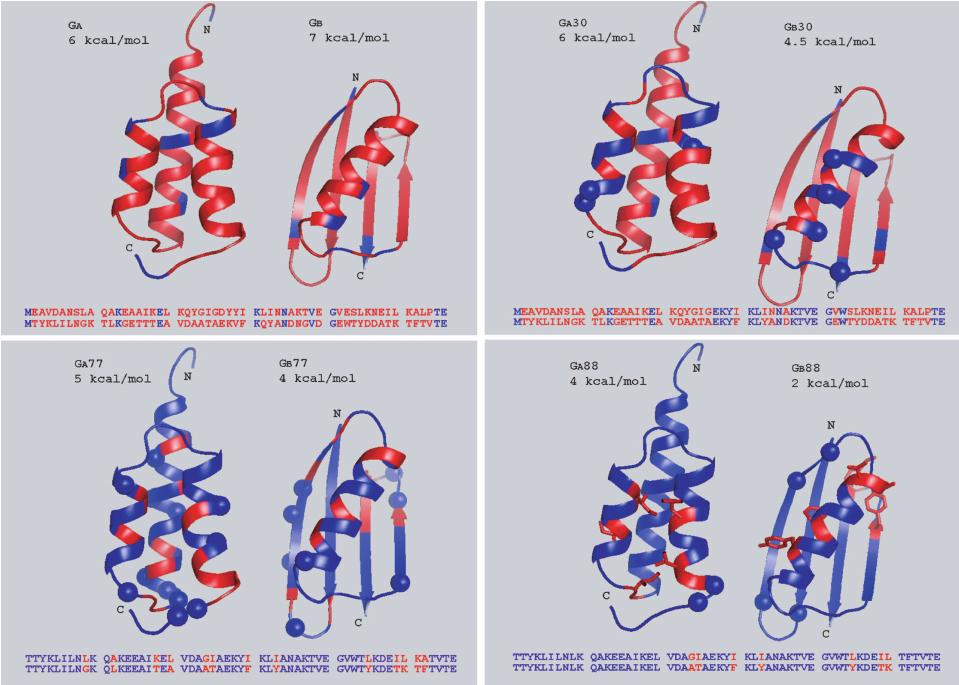
\includegraphics[width=1.0\textwidth]{figures/ga_gb.jpg}
  \caption{Figura representando o design dos domínios. Os resíduos em azul são as mutações introduzidas, esses resíduos são idênticos em ambas as sequências. Em vermelho estão os resíduos diferentes (Figura extraída de \cite{Alexander2007})}
        \label{fig:ga_gb}
\end{figure}

Posteriormente, uma série de outros estudos sobre esses dois domínios demonstrou ser possível obter os dois enovelamentos com idetidade sequencial ainda maiores \cite{He2008,Alexander2009}, até que em 2012, He e colaboradores \cite{He2012}, obtiveram mutações pontuais capazes de alterar a estrutura entre os dois enovelamentos (Figura \ref{fig:camaleonicas}). As estruturas resolvidas por RMN das quatro proteínas foram as utilizadas para compor esse conjunto de dados (PDB IDs: 2LHC, 2LHD, 2LHE, 2LHG) utilizando os 10 primeiros modelos de cada estruturas com o objetivo de manter os dados balanceados.

\begin{figure}
  \centering
  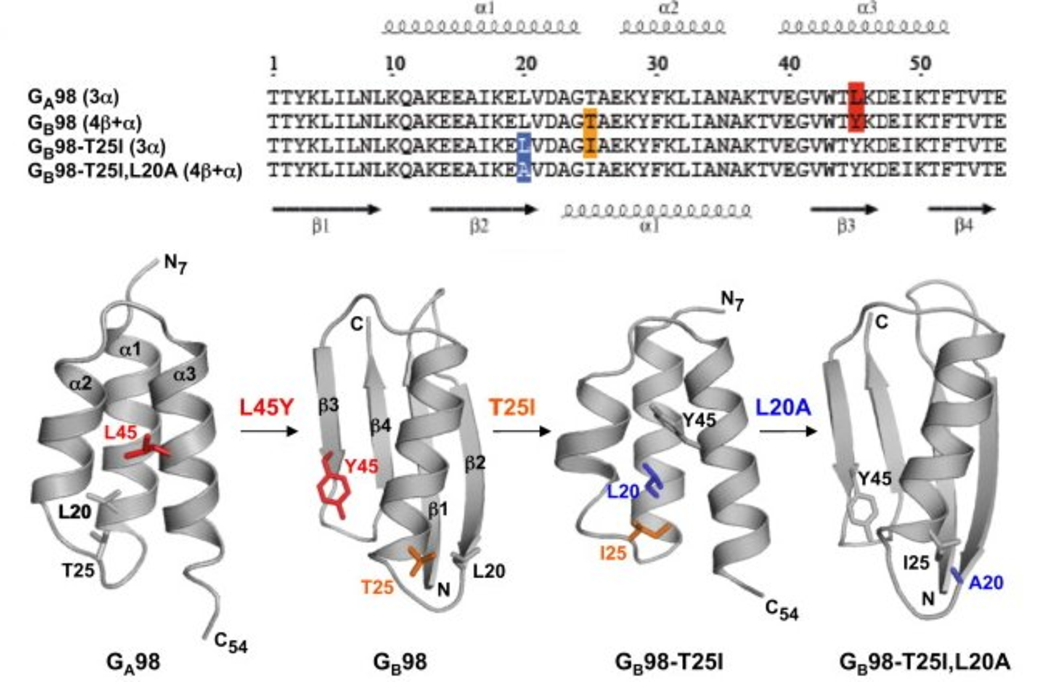
\includegraphics[width=1.0\textwidth]{figures/chameleonic_resume.pdf}
  \caption{Alinhamento das sequências de resíduos mostrando as mutaçoões que ocasionaram as mudanças entre as topologias $3\alpha$ e $4\alpha+\beta$ e os modelos estruturas indicando as posições das mutações (Figura adaptada de \cite{He2012})}
        \label{fig:camaleonicas}
\end{figure}
 
\chapter{Implementação}

\section{Autômato celular}

\subsection{Modelo inicial}

O autômato celular inicialmente proposto possui 24 estados discretos. Esses estados correspondem aos 20 aminoácidos, aos 3 elementos de estruturas secundárias (hélice, fita e random coil) e mais um estado que indica o início/fim da cadeia polipeptídica (\textit{estado=\#}). A vizinhança deste autômato celular é igual a 1 (\textit{r}=1),  o que indica que as regras de transição são dependentes dos dois vizinhos mais próximos, um a esquerda e um a direita. Cada transição pode ocorrer para apenas quatro estados, ou um dos 3 estados que representam os elementos de estrutura secundária ou para o resíduo presente naquela posição da cadeia polipeptídica.

Logo, temos que o total de elementos na regra desse autômato é $24^3$ ou 13824, das quais 24 são elementos estáticos, pois células no estado \textit{\#} sempre permanecerão nesse estado durante a evolução do autômato. Assim temos $4^{24^3-24}$ regras possíveis para esse autômato celular.

\subsection{Modelos extendidos}

Uma das limitações do modelo proposto inicialmente é a perda de informação que ocorre durante a evolução do autômato celular quando as células transitam de estados correpondentes aos aminoácidos para estados de elementos de estrutura secundária. Por exemplo, quando uma lisina evolui para uma hélice, o estado de hélice não possui mais a informação de qual aminoácido havia naquela posição. Acreditamos que essa perda de informação possa ser um fator crítico para o modelo. Consequentemente, avaliamos modelos alternativos que pudessem manter essa informação. 

Uma possibilidade seria manter a informação do resíduo juntamente com o elemento de estrutura secundária. Esse modelo teria 20 estados para os aminoácidos, 20 estados para hélices (um estado diferente para cada aminoácido), 20 estados para fitas e 20 estados para random coils, além do estado de início/fim da cadeia polipeptídica, totalizando 81 estados. Cada regra para esse autômato celular teria $81^3$  ou 531441 elementos, o que seria aproximadamente 38 vezes maior que uma regra do modelo proposto inicialmente, resultando em um aumento significativo da complexidade e, consequentemente, da dificuldade na busca por regras que reproduzam o padrão desejado. Esse aumento de complexidade nos levou a descartar este modelo.

Assim, a alternativa escolhida foi utilizar características dos aminoácidos que mantivessem parcialmente a informação do resíduo durante a evolução do autômato celular, mas sem resultar em um aumento tão elevado do número de regras em relação ao modelo inicial. O primeiro modelo concebido que atende esses requisitos utiliza as características de hidrofobicidade dos aminoácidos. Isso resulta em modelo com 27 estados, sendo dois estados para cada um dos 3 elemento de estrutura secundária, mais os 20 aminoácidos e o início/fim da cadeia polipeptídica. No total, a regra deste autômato celular é formada por  $27^3$, ou 19683, elementos, sendo aproximadamente 1,42 vezes maior que a regra do modelo inicial.

Além deste modelo extendido, dois outros modelos foram utilizados. Um deles adicionando estados para diferenciar glicinas e prolinas, e outro acrescentando estados para diferencia resíduos com cargas positivas e negativas assim como glicinas e prolinas. Ambos utilizam também a hidrofobicidade dos demais resíduos. As regras para esses modelos apresentam  respectivamente $33^3$ e $39^3$ elementos, o que corresponde a um aumento aproximado de 2,6 e 4,3 vezes em relação ao modelo inicial. 

A motivação para o uso da hidrofobicidade dos resíduos foi influenciada por trabalhos de Hecht e colaboradores \cite{Xiong07, West1995} que examinaram a influência de padrões periódicos de hidrofobicidade nas sequências proteicas e sua relação com elementos de estruturas secundárias, concluindo que alguns padrões apresentam preferência por hélices $\alpha$ enquanto outros padrões apresentam preferência por fitas $\beta$ \cite{West1995}.

Em todos os modelos extendidos cada elemento da regra continua com a possibilidade de transitar para apenas 4 estados, ou um dos 3 elementos de estrutura secundária ou o resíduo encontrado naquela posição da cadeia polipeptídica.

\section{EDA}

A busca por regras de um autômato celular que reproduzam um padrão específico, conhecido como problema inverso, é um problema de otimização. Na literatura, esse problema é normalmente abordado utilizando metaheurísticas como algoritmos genéticos ou anelamento simulado (\textit{simulated annealing}). Neste trabalho optamos por utilizar o Algoritmo de Estimação de Distribuição (EDA). Os fatores que determinaram a utilização desse algoritmo foram a facilidade de implementação do EDA de forma distribuída e o pequeno número de parâmetros em relação à algoritmos genéticos.

No EDA distribuído implementado neste trabalho cada elemento da regra do autômato celular, com excessão dos elementos onde a célula apresenta o estado início/fim da cadeia polipeptídica (\textit{estado=\#}),  tem a mesma probabilidade inicial ($p=0,25$) para cada um dos 4 estados de transição. A probabilidade é distribuída pelo nó mestre para os nós escravos. Os nós escravos utilizam a probabilidade recebida para gerar $c \ge 2 $ regras candidatas. As regras candidatas são então utilizadas para evoluir o autômato celular por $t$ passos. Após a evolução, um valor de fitness é atribuído a cada regra. Em seguida, um torneio entre as regras candidatas geradas no nó escravo e a regra com maior fitness é enviada ao nó mestre. Ao recever as $n/c$ regras vencedoras, onde $n$ é o tamanho da população do EDA, o nó mestre atualiza a probabilidade e começa a distribuí-la para os nós escravos, iniciando assim a geração $T+1$ do EDA. A otimização termina após um número específicos de gerações ou quando a probabilidade converge.

\subsection{Função de fitness}

A função de fitness utilizada pelo EDA baseia-se na porcentagem de estados corretos durante a evolução do autômato celular ($t_1 \rightarrow t_{final}$) e estados corretos são os elementos de estrutura secundária idênticos ao concenso obtido entre os quatro métodos de atribuição de estruturas secundária. Quando não há concenso entre os métodos de atribuição de estrutura secundária, a posição é descartada pela função de fitness.   

fitness = 

\section{Implementação}

Tanto o autômato celular quanto o EDA foram implementados na linguagem de programação Go. A estrada do nó mestre é um arquivo de configuração no formato TOML que contém os parâmetros para o autômato celular, o EDA e os dados a serem utilizados. Os dados, ou seja as sequências de aminoácidos das proteínas e suas respectivas estruturas secundárias, são armazenados em um banco de dados chave/valor. A comunicação entre os nós escravo e o nó mestre é feita utilizando chamadas remotas de procedimento (RPC). O código fonte está acessível publicamente no GitHub (\href{https://github.com/jgcarvalho/zeca-search}{github.com/jgcarvalho/zeca-search}, \href{https://github.com/jgcarvalho/zeca-search-master}{zeca-search-master} e \href{https://github.com/jgcarvalho/zeca-search-slave}{zeca-search-slave})  



\cleardoublepage
\part{Resultados}
\chapter{Análise dos dados}

\chapter{Aprendizado de regras de transição}

Nas seções seguintes mostraremos resultados da capacidade de autômatos celulares reproduzirem padrões de estruturas secundárias a partir da sequência de aminoácidos e da utilização do EDA para buscar regras de transição. Inicialmente, discutiremos os autômatos celulares e as diferentes opções de estados utilizados. Em seguida, discutiremos os resultados da otimização das regras de transição utilizando um EDA distribuído.  

%Nas seções de resultados a seguir mostraremos a capacidade do EDA em gerar um conjunto de regras de transição  para o autômato celular que permitiu a construção de um preditor de estruturas secundárias capaz de identificar a mudança de poucos aminoácidos na sequencia em contraste com grandes modificações das estruturas secundárias em proteínas camaleônicas. Também, ....

\section{Autômato celular}

Os modelos de autômatos celulares foram testados, até o momento, no conjunto de proteínas com alta identidade sequencial, mas com grandes diferenças de estrutura secundária, o que o torna um problema desafiador. A escolha desse conjunto para os testes dos autômatos celulares baseou-se, também, na facilidade de analisar e visualizar a formação e propagação dos elementos de estruturas secundárias nessas proteínas, pelo fato de serem pequenas.

%A comparação entre os modelos de autômatos celulares foram realizadas primeiramente, e até o momento, apenas no conjunto de proteínas com alta identidade sequencial. A escolha desse conjunto para os testes dos autômatos celulares baseou-se na facilidade de observar e analisar a formação e propagação dos elementos de estruturas secundárias nessas proteínas. É importante ressaltar que ao otimizarmos as regras de transição para este conjunto restrito de proteínas, nosso objetivo é avaliar a capacidade dos modelos propostos de autômatos celulares em recuperar corretamente a estrutura secundária atribuída aos resíduos.   

O modelo idealizado para o autômato celular deveria ter a capacidade de propagar sinais locais ao longo da sequência, e assim, resultar na formação de padrões globais. Tal capacidade está relacionada aos estados que ocorrem durante a evolução do autômato celular, sendo dependentes do número de estados possíveis e também do tamanho da vizinhança utilizada. Como todos os autômatos celulares propostos tem vizinhança 1 (Seção \ref{sssec:ca}), a capacidade de formar e propagar os sinais será dependente apenas dos estados possíveis do autômato celular.

%PSLO Zé essa frase está um pouco confusa: "Como todos os autômatos celulares propostos tem vizinhança 1 (um) por questões de complexidade (ver ref metodos), a capacidade de formar e propagar os sinais será dependente apenas dos estados possíveis do autômato celular."

%Ao otimizarmos as regras apenas para 

Entre os quatro modelos testados, o número de estados para os elementos de estrutura secundária demonstrou relação com a acurácia do modelo. Assim, CAs com estados de elementos de estrutura secundária que conservam mais características dos resíduos mostraram-se mais promissores (Figura \ref{fig:ca_errors}).

\begin{figure}
  \centering
  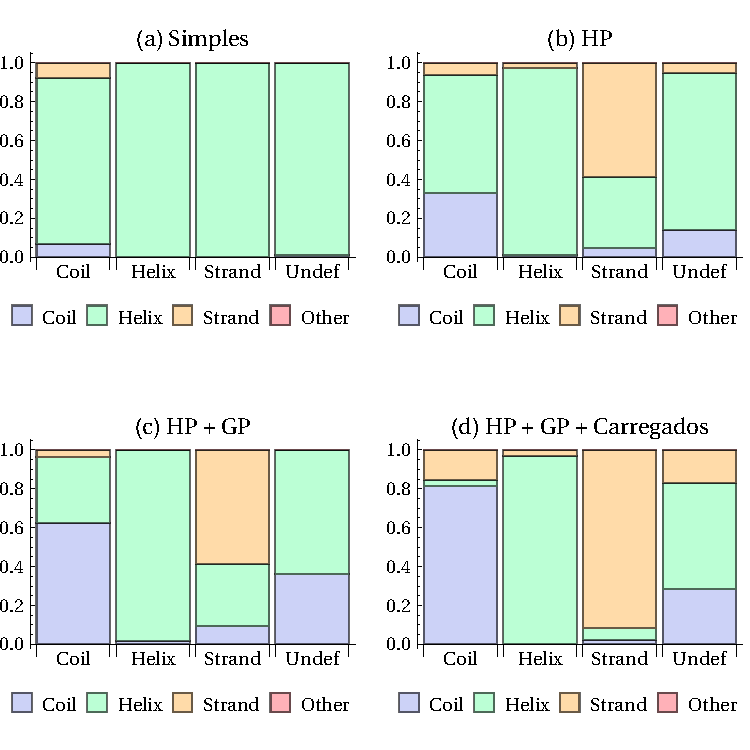
\includegraphics[width=.9\textwidth]{figures/chamel_errors_ca.pdf}
  \caption{Comparação de autômatos celulares com diferentes estados. O gráfico mostra proporção de elementos preditos para cada um dos elementos da estrutura experimental. Em (a) os resultados obtidos por um autômato celular que utiliza apenas 3 estados (H,E,C) para as estruturas secundárias. Em (b) um autômato que apresenta 6 estados, acrescentando as características de hidrofobicidade do resíduo (hidrofóbico/hidrofílico) aos estados de estrutura secundária. Em (c), um autômato celular que apresenta 12 estados após a adição de Gly e Pro como características especias das estruturas secundárias. E por fim, em (d), um autômato celular com 18 estados para as estruturas secundárias onde os estados carregam as características hidrofóbico, hidrofílico, glicina, prolina e resíduos carregados positivamente e negativamente.} 
        \label{fig:ca_errors}
\end{figure}

\begin{figure}
  \centering
  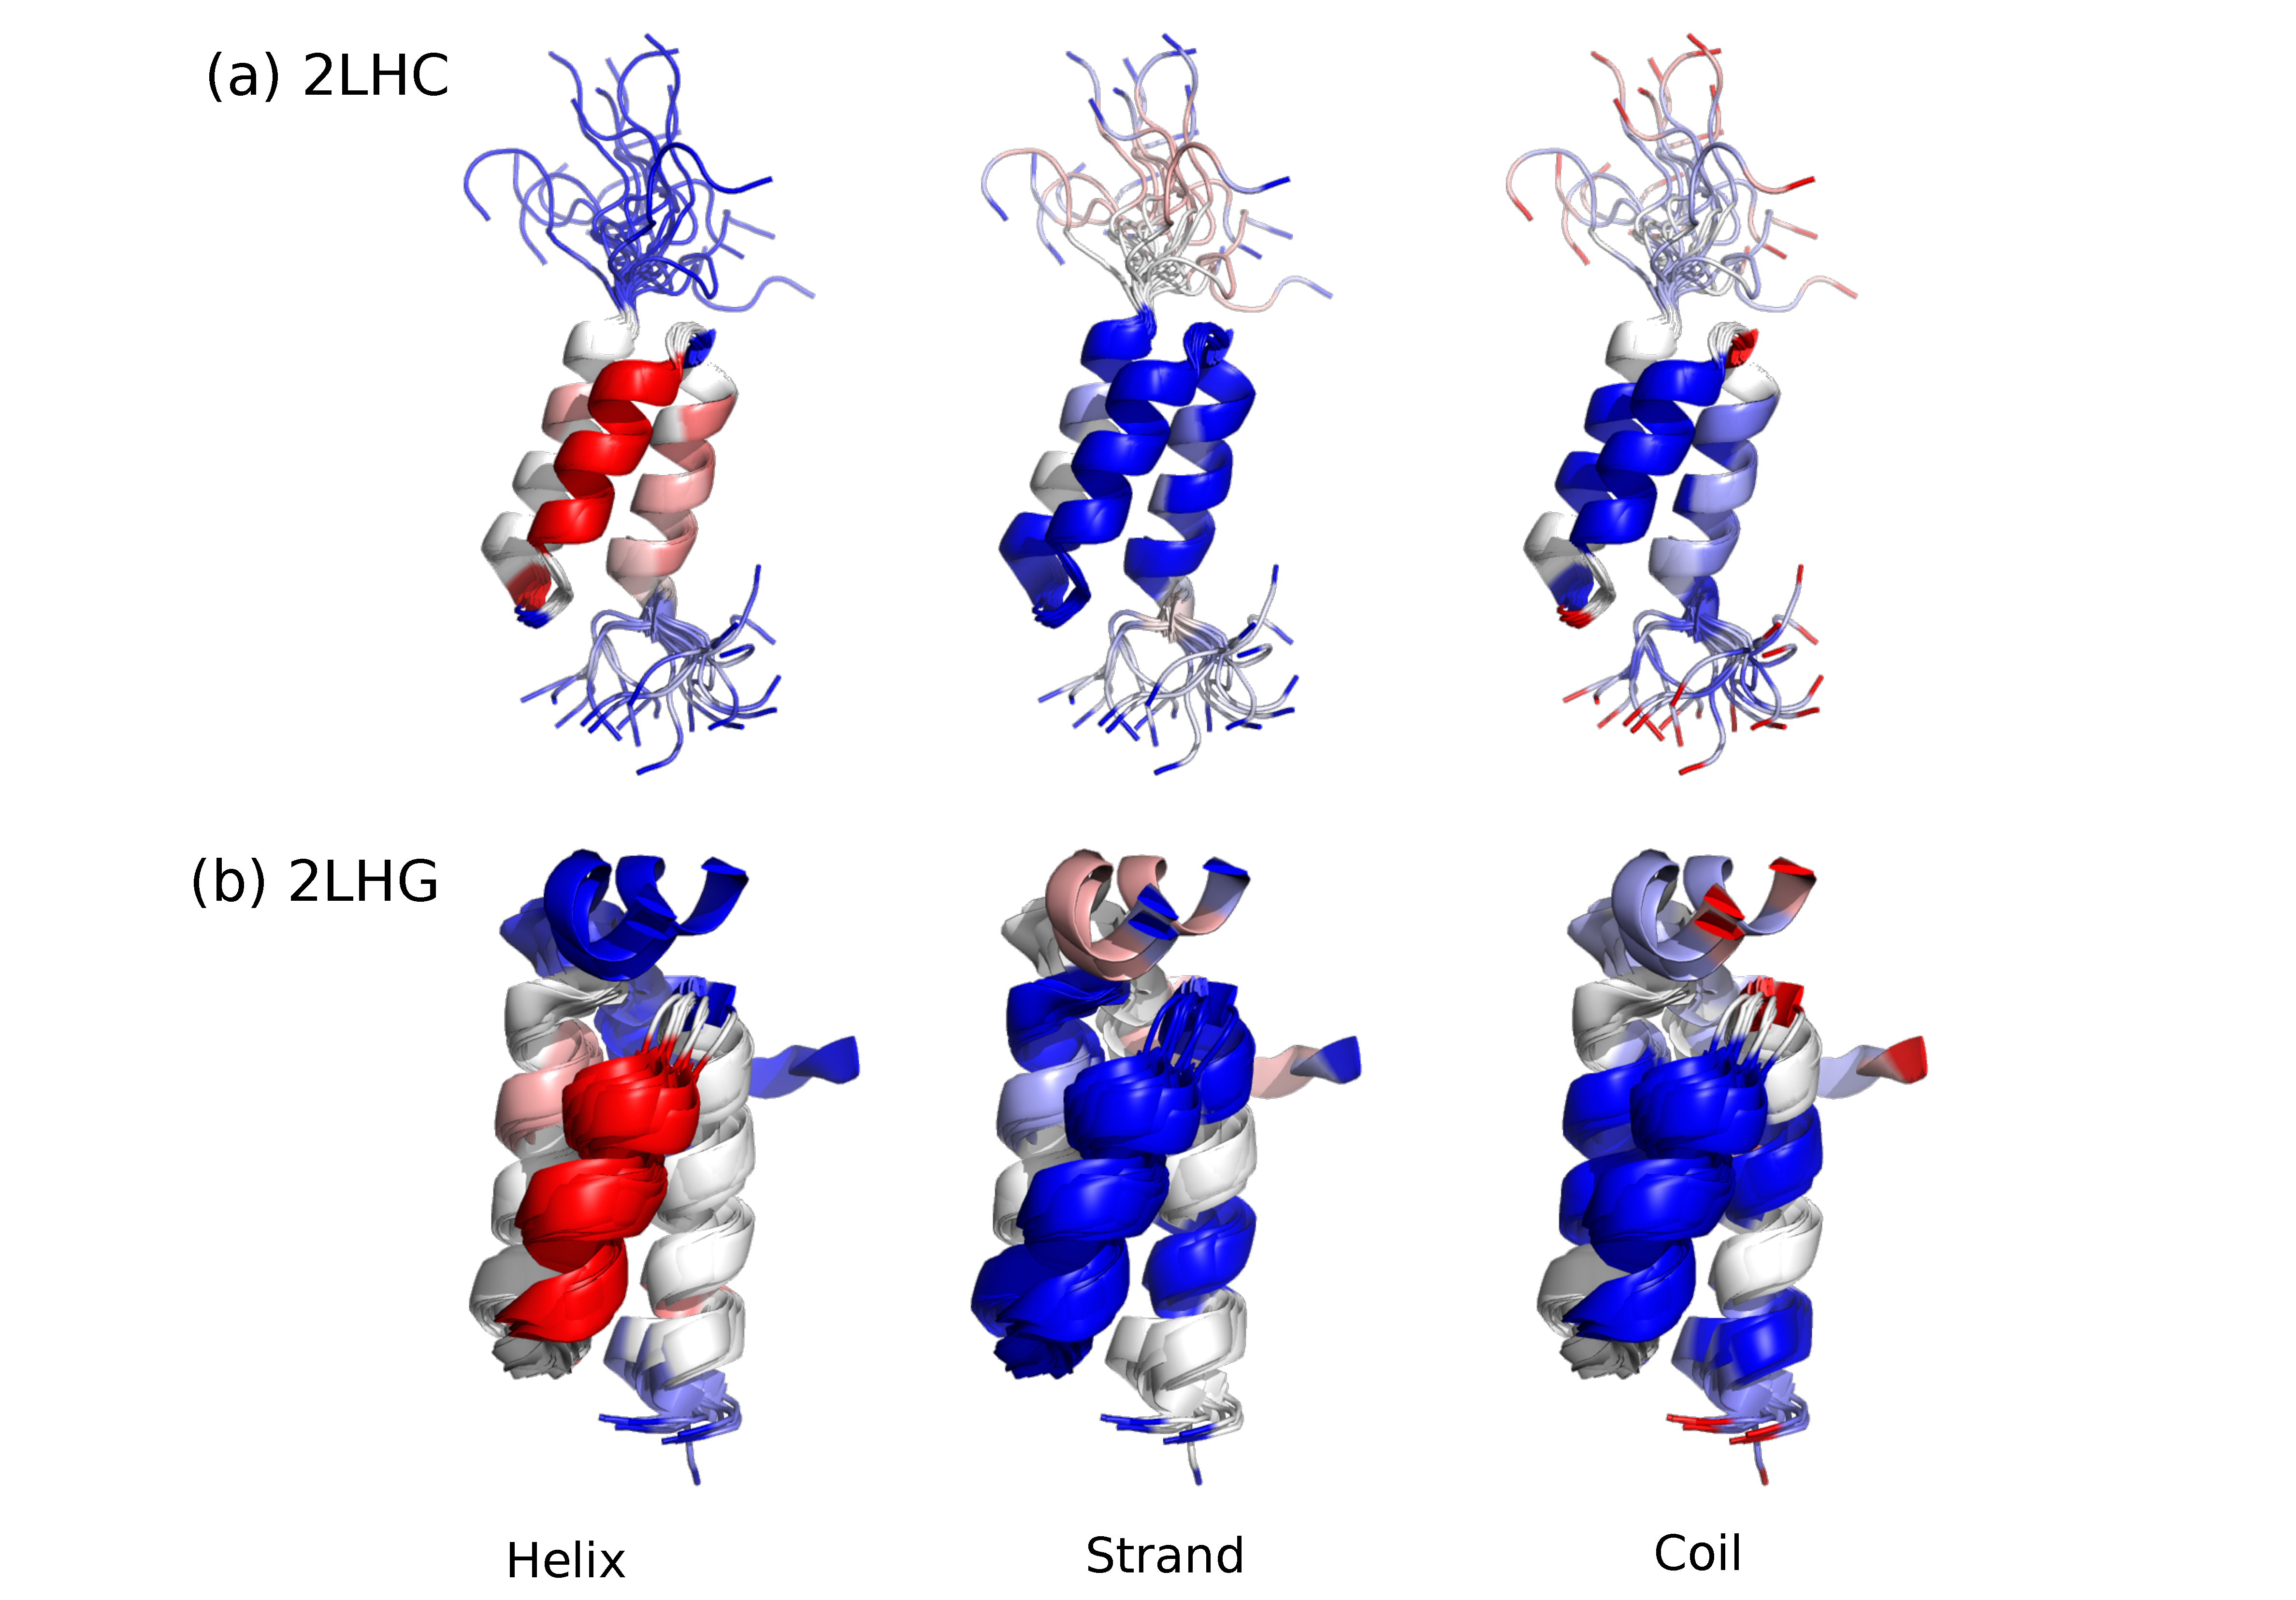
\includegraphics[width=1\textwidth]{figures/camel_2lhc_2lhg.pdf}
  \caption{Modelos estruturais das proteínas Ga98 (PDB ID: 2LHC) e GB98-T25I (PDB ID: 2LHG) que possuem a topologia de feixe de hélices alpha. As cores representam as frequências dos estados durante a evolução do autômato celular num gradiente do vermelho, 100\%, ao azul, 0\%. Cada elemento de estrutura secundária (hélice, fita e coil) corresponde a uma coluna da figura. Notamos que a hélice 2 (intermediária) demonstra alta frequência do estado de hélice no autômato celular após 10000 passos. As outras duas hélices apresentam frequências menores em relação a hélice 2, mas maiores que os outros estados. Entre os resíduos de conexão entre as hélices, aparecem alguns com grande frequência de estados coil. Nas regiões N e C terminais, há uma maior frequência de fitas e coils, em relação à hélices. O autômato celular utilizado possui os estados HP+GP+Carregados.}
        \label{fig:camel_2lhc_2lhg}
\end{figure}

\begin{figure}
  \centering
  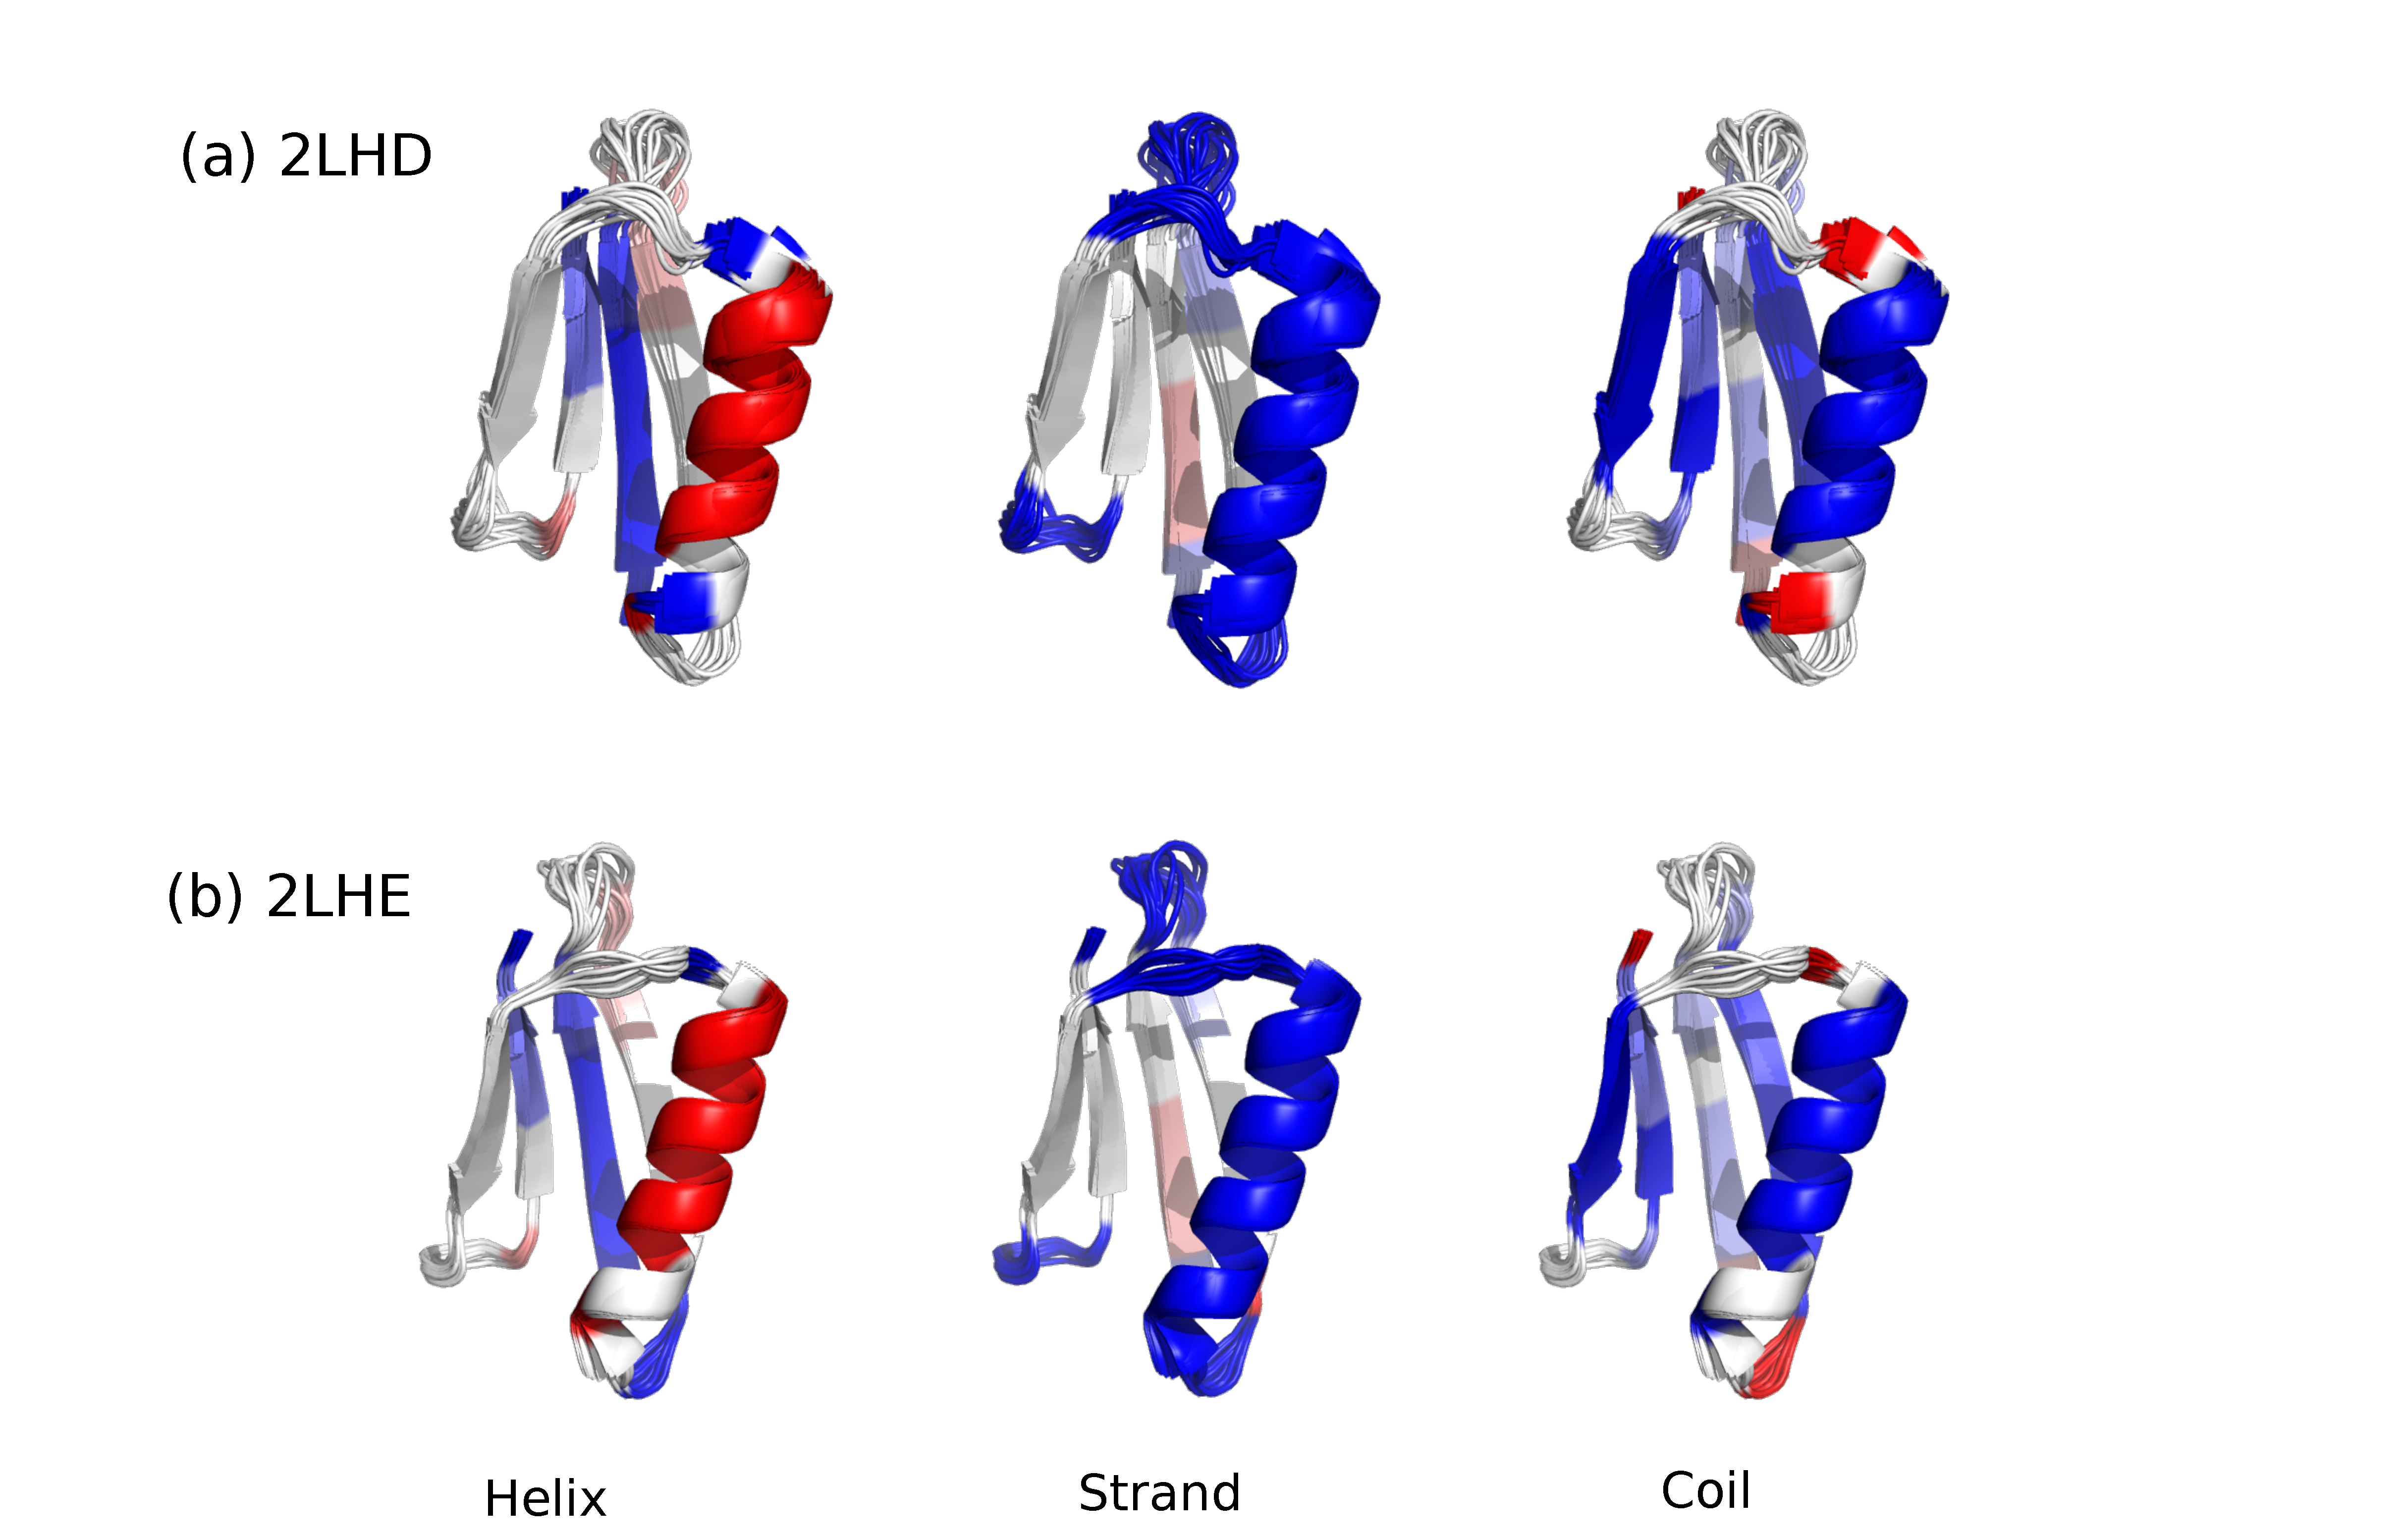
\includegraphics[width=1\textwidth]{figures/camel_2lhd_2lhe.pdf}
  \caption{Modelos estruturais das proteínas GB98 (PDB ID: 2LHD) e GB98-T25I,L20A (PDB ID: 2LHE) que apresentam a topologia de 4 fitas beta e hélice alpha. As cores representam as frequências dos estados durante a evolução do autômato celular num gradiente do vermelho, 100\%, ao azul, 0\%. Cada elemento de estrutura secundária (hélice, fita e coil) corresponde a uma coluna da figura. Notamos que a hélice demonstra alta frequência do estado de hélice no autômato celular após 10000 passos. As fitas apresentam uma frequência tanto estados de hélices como de fitas, exceto a fita 1 que apresenta baixa frequência de hélices e maior frequência de fitas. A regiões de conexão entre as fitas e da hélice com as fitas apresentam maior frequência de coils. O autômato celular utilizado possui os estados HP+GP+Carregados.}
        \label{fig:camel_2lhd_2lhe}
\end{figure}


\section{Análise do desempenho do EDA implementado}

O aprendizado das regras realizado através de um algoritmo de EDA distribuído demonstrou-se eficiente dado a complexidade do problema. Utilizando sete nós (448 núcleos) no cluster de computação de alto desempenho EMU-2 (adquirido pelo "Programa de Equipamento  Multiusuário da FAPESP-2009", 2009/53853-5, localizado no Centro Internacional de Pesquisa e Ensino do Hospital A. C. Camargo em  São Paulo) foi possível evoluir o EDA com 10000 indivíduos por 1000 gerações em pouco menos de duas semanas.

Cada nó de trabalho apresentou um uso de memória de 75\% (48 GB), e manteve o processamento próximo a 100\% por núcleo (1.6 GHz). O mecanismo de comunicação por RPC entre o nó mestre e os nós de trabalho não sobrecarregou a rede (1Gbs). Isso nos permite concluir que o algoritmo é escalável em clusters com maior número de nós e processadores de maior desempenho.

A opção por realizar o torneio entre soluções candidatas nos nós de trabalho, permite apenas a opção de realizar o torneio entre as k últimas soluções geradas no próprio nó. Consequentemente, as k-1 soluções perdedoras são descartadas, havendo portanto, a remoção das soluções perdedoras em cada torneio. 

Usualmente, o método de seleção por torneio utilizado em algoritmos genéticos não distribuídos acumula as solução candidatas até atingir o tamanho máximo populacional, quando então, é realizado o torneio. Isso permite que o torneio seja feito sem a eliminação dos perdedores, possibilitando que a seleção destes ocorram em outros combates.

Entretanto, no EDA distribuído, para aplicarmos um torneio sem eliminação dos perdedores seria necessário:

\begin{enumerate}
	\item o envio de todas as soluções candidatas para o nó mestre, o que resultaria em maior consumo de rede;
	\item o acúmulo de todas as soluções candidatas até atingir o tamanho máximo da população, gerando uma limitação da memória disponível;
	\item a espera até a realização do torneio para iniciar o cálculo das probabilidades, resultando no aumento do tempo ocioso nos nós de trabalho igual ao intervalo de tempo do envio da última solução até a finalização do cálculo das probabilidades.
\end{enumerate} 

A escolha em realizar o torneio nos nós de trabalho demonstrou ser escalável, manter a variabilidade das soluções candidatas ao longo da evolução e convergência (Figura \ref{fig:evo_eda}).

\begin{figure}
  \centering
  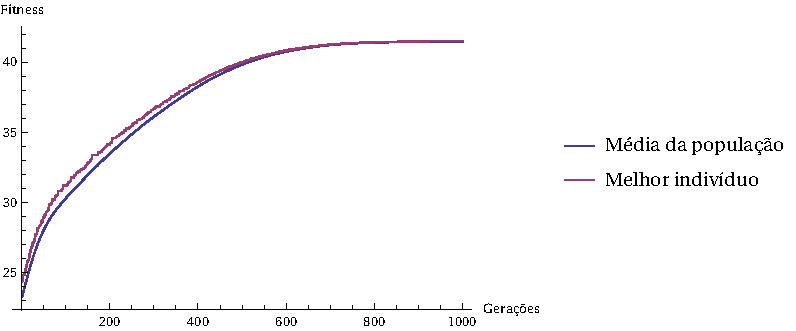
\includegraphics[width=1\textwidth]{figures/evo_Eda.pdf}
  \caption{Gráfico que representa a pontuação (\textit{fitness}) média da população de regras candidatas e da melhor regra ao longo de 1000 gerações do EDA.}
        \label{fig:evo_eda}
\end{figure}

\subsection{Deriva genética}

A evolução do EDA por 1000 gerações com torneio de dois (k=2) e população de 10000 indivíduos, demonstrou sinais de deriva genética a partir de 564 gerações. Tais sinais podem ser detectados observando-se as probabilidades dos 38 elementos de regra que não ocorrem no conjunto de proteínas. Esses elementos são do tipo [\#][\textit{x}][\#].

Os elementos [\#][\textit{x}][\#], onde o \textit{x} correponde a qualquer estado exceto [\#], não apresentam probabilidade fixa, mas também, por estarem ausentes nas proteínas, não sofrem pressão seletiva. Logo, suas variações são aleatórias.

Na geração 564 um desses 38 elementos apresentou probabilidade zero ($p=0$), de transitar para um dos quatro estados possíveis, indicando a eliminação de um gene da população por deriva genética. Ao final das 1000 gerações 11 dos 38 elementos apresentavam probabilidade zero para uma das transições (Figura \ref{fig:deriva_genetica}).

%PSLO Zé vc pode trabalhar um pouco mais no texto dessa seção. Eu pelo menos não achei as conclusões muito óbvias

\begin{figure}
  \centering
  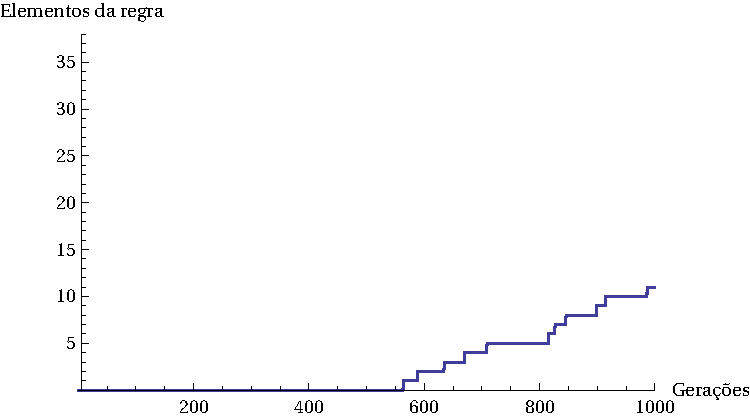
\includegraphics[width=1\textwidth]{figures/deriva_genetica.pdf}
  \caption{Gráfico que indica efeitos de deriva genética através da amostragem de 38 elementos que não sofrem pressão seletiva proveniente do \textit{fitness}. Na geração 564, um desses elementos apresentou probabilidade igual a zero para uma das transições. Ao final das 1000 gerações, 11 elementos apresentam probabilidade zero para ao menos um dos estados.}
        \label{fig:deriva_genetica}
\end{figure}

% PSLO Zé vamos tentar usar uma tradução para fitness. Senão me engano no capítulo 5 sugeri função de pontuação dos individuos


\subsection{Função de pontuação dos indivíduos}

A simplicidade da função de pontuação dos indivíduos (Equação \ref{eq:fitness}) demonstrou problemas que acreditamos serem solucionáveis na continuação deste trabalho. Um desses problemas é ocasionado pelo desbalanceamento dos dados de treinamento (Figura \ref{fig:occ_ss}). 

\begin{figure}
  \centering
  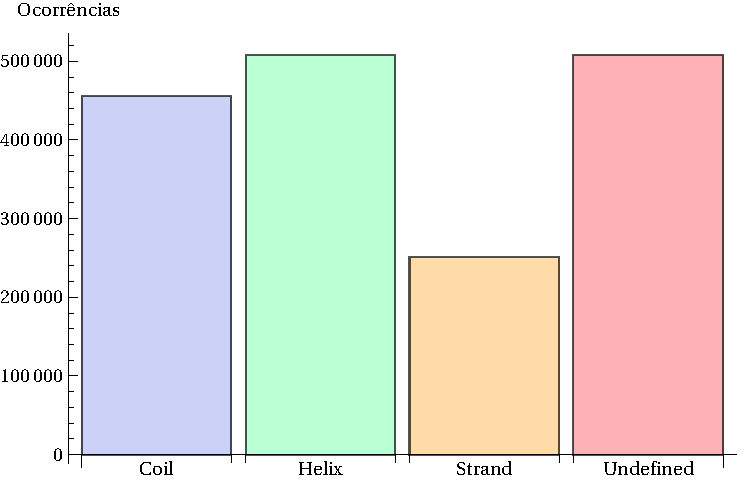
\includegraphics[width=0.9\textwidth]{figures/occ_ss.pdf}
  \caption{Desbalanceamento dos elementos de estrutura secundária no conjunto de dados.}
        \label{fig:occ_ss}
\end{figure}

Os resultados obtidos indicam uma maior acurácia para os elementos de estrutura secundária mais frequentes no conjunto de treinamento. Esse é um problema recorrente no aprendizado com classes desbalanceadas e costuma ser tratado na função de pontuação (\textit{fitness}) (Figura \ref{fig:q3}), por exemplo, utilizando funções que considerem a acurácia por classes. As alterações na função de pontuação para tratar este problema são preferiveis em relação à modificações no conjunto de dados para equilibrar as classes, uma vez que modificações no conjunto de dados envolveriam a retirada de informação de classes mais frequentes ou a duplicação de informação das classes menos frequentes, ambas produzindo consequências distorcivas na informação presente no conjunto de treinamento.

%\begin{figure}
%  \centering
%  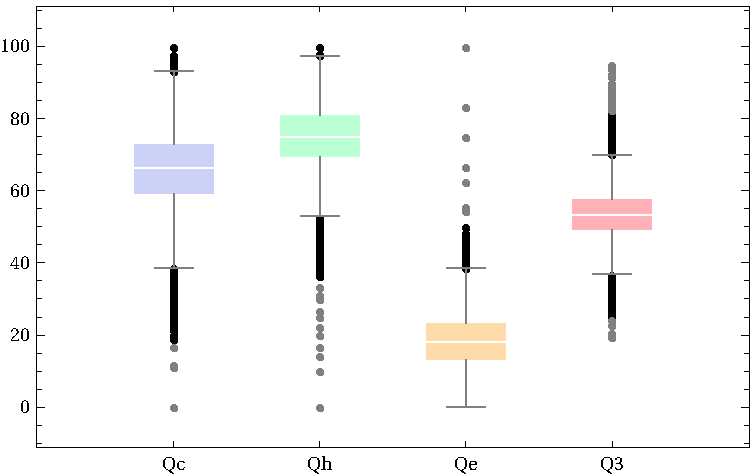
\includegraphics[width=0.9\textwidth]{figures/q3.pdf}
%  \caption{q3}
%        \label{fig:q3}
%\end{figure}

% Avaliamos também se havia alguma relação aparente dos elementos preditos com os ângulos phi e psi do resíduos, o que poderia justificar parcilamente  erros nos elementos preditos. Entretanto, aparentemente não existe tal relação (figuras).



% Roc curve

%Outra modificação possível na função de fitness seria buscar a maximização da frequência dos estados durante a evolução do autômato.  

\subsection{Fatores que influenciam no método de seleção do EDA}

O número de ocorrências de trincas de aminoácidos no conjunto de proteínas apresentou grande variação (Figura \ref{fig:histograma_occ}). Para avaliar a influência dessa variação no EDA nós procuramos por correlações entre fatores que poderiam influenciar na seleção.

\begin{figure}
  \centering
  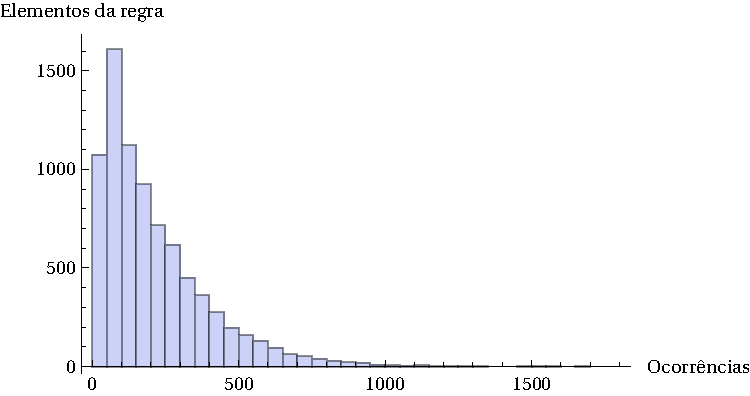
\includegraphics[width=1\textwidth]{figures/histograma_occ.pdf}
  \caption{Histograma de ocorrencia das trincas}
        \label{fig:histograma_occ}
\end{figure}

\begin{table}
\begin{tabular}{cc}
\toprule
\tableheadline{Trinca} & \tableheadline{Frequência}\\
\midrule
CCW & 2\\
CMW & 2\\
WMC & 2\\
WPC & 3\\
WCW & 3\\
CHW & 4\\
\bottomrule
\end{tabular}
\quad
\begin{tabular}{cc}
\toprule
\tableheadline{Trinca} & \tableheadline{Frequência}\\
\midrule
EAL & 1316\\
LAA & 1478\\
AAL & 1534\\
ALA & 1563\\
AAA & 1682\\
HHH & 6143\\
\bottomrule
\end{tabular}
\caption{Trincas de aminoácidos menos (à esquerda) e mais (à direita) frequentes no conjunto de treinamento.}
\end{table}



A figura \ref{fig:probG999_occXprob} representa a distribuição das probabilidades máximas e mínimas dos elementos da regra em relação a frequência de ocorrência das trincas de aminoácidos no conjunto. O gráfico e o valor de correlação (Spearman = 0.09) entre as probabilidades e a frequência de ocorrência das trincas, indica não haver uma grande influência da frequência das trincas durante a seleção.	

%incluir as figuras do anexo

\begin{figure}
  \centering
  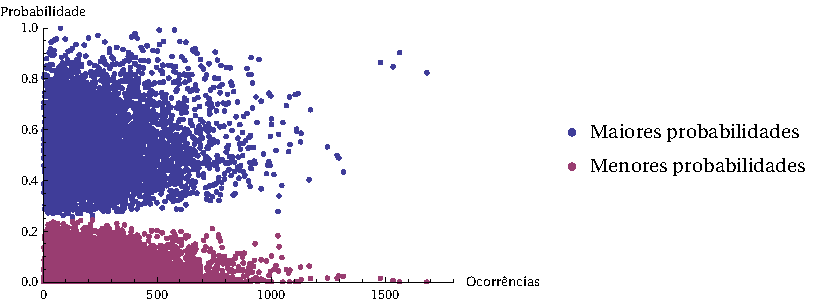
\includegraphics[width=1\textwidth]{figures/probG999_occXprob.pdf}
  \caption{Probabilidades máximas e mínimas dos elementos da regra de transição em relação ao número de ocorrência das trincas de aminoácidos.}
        \label{fig:probG999_occXprob}
\end{figure}


Outros fatores que poderiam influenciar a evolução do EDA seriam: \textit{(1)} a probabilidade da trinca ser observada em uma determinada estrutura secundária; \textit{(2)} o número de ocorrências da trinca em determinada estrutura secundária; \textit{(3)} a taxa de acertos por trincas para determinada estrutura secundária. 

%ta estranho essa parte    

As probabilidades de transição dos elementos da regra (EDA), não apresentam aparente relação com as proporções encontradas para cada estrutura secundária nas trincas (Figura \ref{fig:relacao_prob_propss}). Assim como não apresentaram relação com a frequência de ocorrências de determinada estrutura para uma trinca ou com a proporção de trincas corretamente classificadas por estrutura secundária. 

%PSLO Para uma taxa de acertos maior eu deveria esperar que acontece uma correlação alta entre a probabilidade gerada pelo EDA para uma dada regra para uma certa estrutura secundaria específica.   



\begin{figure}
  \centering
  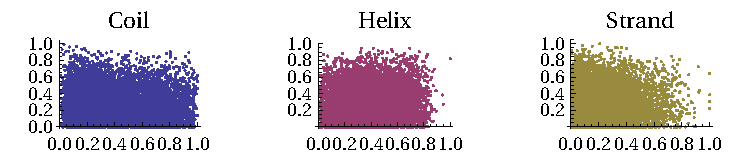
\includegraphics[width=1\textwidth]{figures/relacao_prob_propss.pdf}
  \caption{Relação entre a proporção de uma trinca de aminoácidos em determinada estrutura secundária e a probabilidade resultante da otimização utilizando EDA.}
        \label{fig:relacao_prob_propss}
\end{figure}

A ausência da primeira relação (probabilidade do EDA x propensão de estruturas secundárias por trinca) pode indicar que as probabilidades de transição dos demais elementos da regra e sua aplicação ao longo da evolução do CA estão propagando as probabilidades e sofrendo influência da vizinhança na busca por produzir estruturas secundárias mais próximas as reais. 

Entretanto, observamos uma relação entre a proporção de elementos de estruturas secundárias para um trinca e a proporção de acertos da trinca para a mesma estrutura secundária. Acreditamos que isso seja um indício que o aprendizado, ou otimização da regra, precisa ser melhorado para que elementos de estruturas secundárias menos comuns a determinadas trincas possam ser corretamente preditos (Figura  \ref{fig:prop_acerto} e Tabela \ref{tab:corr_acertos}).  


Há também uma relação menos influente entre o número de ocorrências de uma determinada estrutura secundária nas trincas e a proporção de acertos dessa trinca para a mesma estrutura secundária ((Figura \ref{fig:occ_acerto}) e Tabela \ref{tab:corr_acertos}).

\begin{figure}
  \centering
  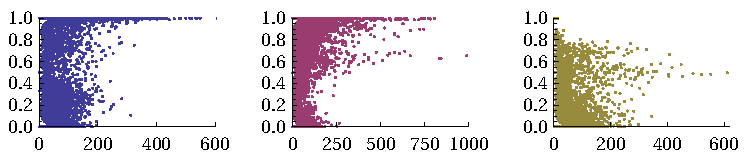
\includegraphics[width=1\textwidth]{figures/occ_acerto.pdf}
  \caption{Relação entre o número de ocorrências das estruturas secundárias por trincas em relação a proporção de resíduos corretamente classificados.}
        \label{fig:occ_acerto}
\end{figure}

\begin{figure}
	\centering
	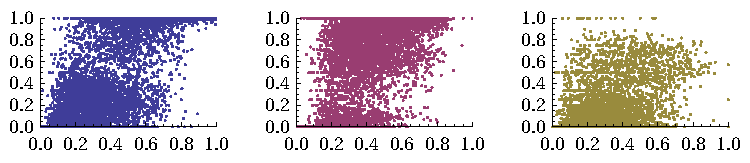
\includegraphics[width=1\textwidth]{figures/prop_acerto.pdf}
	\caption{Relação entre a proporção observada de cada estrutura secundária para as trincas e a proporção de resíduos corretamente classificados.}
	\label{fig:prop_acerto}
\end{figure}

\begin{table}
    \myfloatalign
    \label{tab:corr_acertos}
  \begin{tabularx}{\textwidth}{Xlll} \toprule
    \tableheadline{Correlação}   & \tableheadline{coil}   & \tableheadline{hélices}  & \tableheadline{fitas} \\ 
    \midrule
     Proporção das trincas  & 0,75 & 0,60   & 0,60   \\
    Ocorrências das trincas  & 0,60 & 0,24   & 0,38  \\
    %autem vulputate ex & parola & romanic \\
    %usu mucius iisque & studio & sanctificatef \\
    \bottomrule
  \end{tabularx}
  \caption{Correlação (Spearman) entre a proporção de acertos na predição e: (1) proporção das trincas nas estruturas secundárias, (2) número de ocorrências das trincas nas estruturas secundárias}
\end{table}

Ambas as relações encontradas eram esperadas, pois indicam uma tendência do método a privilegiar o aprendizado, ou otimização, de elementos capazes de influenciar com maior intensidade a função de \textit{fitness}. Isso mostra a importância de manter um variabilidade alta na população e reduzir efeitos de deriva genética para que a otimização escape de mínimos locais e consiga aprender, também, as probabilidades para trincas menos frequentes nas proteínas e/ou com proporções pequenas para determinadas estruturas secundárias.

%\chapter{Aprendizado das regras gerais}




% \section{contagem de aa}
% CCW      2
% CMW      2
% WMC      2
% WPC      3
% WCW      3
% CHW      4
% MWC      4
% CCC      4
% CMC      4
% WCC      4
% CWW      4
% WWM      5
% MCW      5
% CWC      5
% MWM      6
% CCM      6
% MWH      6
% CWH      6
% FWC      6
% QCC      6
% QCW      6
% WWW      6
% WCH      7
% CMM      7
% YCW      7
% WCM      7
% CIW      7
% HWC      7
% CQW      7
% CYW      8
% ..     ...
% AAE   1000
% LKE   1001
% AEA   1011
% EAA   1021
% AGA   1029
% AGL   1032
% AAV   1034
% AEL   1046
% ELA   1051
% EEL   1066
% ALG   1076
% LGL   1080
% LAG   1082
% VAA   1105
% ALE   1111
% LEA   1111
% AVA   1118
% ELL   1129
% LAL   1131
% LLE   1166
% LAE   1172
% AAG   1246
% ALL   1289
% LLA   1296
% EAL   1316
% LAA   1478
% AAL   1534
% ALA   1563
% AAA   1682
% HHH   6143 
\chapter{Aplicação das regras de transição}

Após a otimização das regras de transição utilizando o EDA, nós avaliamos o desempenho das regras em classificar corretamente os elementos de estrutura secundária. A regra de transição que apresentou a melhor acurácia ao longo da evolução do EDA foi utilizada em um autômato celular determinístico, onde cada elemento da regra apresenta sempre a mesma transição.

Além do autômato celular determinístico, nós utilizamos as probabilidades da última geração do EDA como uma regra de transição para um autômato celular probabilístico.  

\section{Autômato celular determinístico}

Q3

curva Roc

\section{Autômato celular probabilístico}

Q3

curva Roc



\part{Perspectivas futuras}
%\addtocontents{toc}{\protect\clearpage} % <--- just debug stuff, ignore
\chapter{Perspectivas futuras}

%Neste capítulo discutiremos alterações que estão sendo planejadas para melhorar o método que estamos desenvolvendo. Essas alterações foram pensadas baseando-se nos resultados obtidos até o momento e nas possibilidades para melhorá-los.

Neste capítulo discutiremos atividades que estão sendo planejadas para melhorar o método de predição de estruturas secundárias usando autômatos celulares. Essas alterações foram pensadas baseando-se nos resultados obtidos até o momento e nas possibilidades para melhorá-los.

\subsection{Função de fitness}

%Os resultados obtidos até o momento indicam que a função de fitness precisa de modificada para cornseguirmos melhorar a acurácia da predição. A função utilizada até o momento não mostrou-se eficaz ao lidar com classes desbalanceadas como podemos notar pela menor acurácia obtida em fitas quando comparada a hélices e coils.

Os resultados obtidos até o momento indicam que a função de fitness precisa ser modificada para conseguirmos melhorar a acurácia da predição. A função utilizada não mostrou-se eficaz ao lidar com classes desbalanceadas como podemos notar pela menor acurácia obtida em fitas quando comparada a hélices e coils.

A ineficácia ao lidar com classes desbalanceadas, não prejudica somente a predição das classes menos numerosas, mas também a das classes mais frequentes, uma vez que essas tendem a ser superestimadas. Diversas abordagens podem ser utilizadas para em casos onde há desbalanceamento das classes como a re-amostragem através da remoção de dados da classe majoritária ou então a duplicação de dados da classe minoritária \cite{Kumar2012}. Outra alternativa seria a alteração da função de fitness para compensar o desbalanceamento.

Acreditamos que a alteração da função de fitness será a estratégia mais adequada neste trabalho, pois evitaria a remoção ou a duplicação de informações do conjunto de dados. Entre as funções de fitness que planejamos testar estão o Coeficiente de Correlação de Matthews (MCC) \cite{Gorodkin2004} e a CBA (\textit{Class Balance Accuracy}) \cite{Mosley2013}.  



%
%\cite{Jurman2010}
%\cite{Jurman2012}



%Descrever ambas as funçoes. 



\subsection{CA probabilístico durante a otimização das regras pelo EDA}

Como descrito anteriormente, durante a otimização, o EDA envia probabilidades para os nós de trabalho que irão gerar regras de transição candidatas que finalmente disputarão os torneios. Atualmente, estas regras de transição geradas nos nós de trabalho são determinísticas. 
 
Uma alternativa que planejamos implementar é a modificação dos autômatos celulares utilizados durante a otimização das regras para autômatos celulares do tipo probabilísticos. Com isso, as probabilidades do EDA não representariam apenas as probabilidades das transições na população do EDA, mas sim a probabilidade de transição do elemento em si. Acreditamos que essa modificação aproximaria as regras de transição de um modelo físico, onde as probabilidades de transição teriam relação com a energia livre de uma transição da trinca de estados. 



% Utilizar um CA probabilistico durante a fase de otimização das regras através do EDA.

% Para alterar as probabilidades, será necessário que probabilidades sofram variação durante a criação de um indivíduo. A variação não devera ser brusca (distribuiçao normal), para manter uma exploração local da regiao. Essa variação podera ser dependente de outros fatores, por exemplo, da propria variação de probabilidades ao longo da evolução do EDA 

\subsection{Predição de estados conformacionais dos resíduos}

Uma possibilidade que está sendo avaliada é modificação do objetivo da predição. A predição de elementos da estrutura secundária por resíduo não apresenta uma correspondente física uma vez que um resíduo raramente compõe isoladamente uma estrutura secundária. Por exemplo, hélices e fitas são formadas pela repetição de resíduos que se encontram em estados conformacionais específicos. Logo, um resíduo isolado no estado conformacional de uma hélice, poderia fazer fazer parte outro elemento de estrutura secundária como um coil ou volta.

Por sua vez, uma estrutura secundária poderia ser classificada pelo estado conformacional dos resíduos, sendo o estado conformacional representado por regiões de ângulos $\phi$ e $\psi$. Assim, ao invés do autômato celular predizer os elementos de estrutura secundária ele poderia predizer estados conformacionais referentes a regiões dos ângulos. 

Esta representação, combinada com o uso de um CA probabilístico, representaria as probabilidades dos estados conformacionais, fornecendo também as alterações de probabilidades que ocorrem ao longo da evolução do autômato celular. Assim, a evolução desse CA probabilístico resultaria na predição das probabilidades de cada aminoácido estar em cada estado conformacional.

Isso traria a vantagem de, além de ser possível descrever os elementos de estrutura secundária utilizando os estados conformacionais de cada resíduo, seria possível obter também informações da estrutura tridimensional das proteínas. Mesmo que essa abordagem diminuísse a acurácia na predição de elementos de estrutura secundária, o ganho de informação que poderíamos na conformação tridimensional, por exemplo, em coils, poderia compensar a mudança para a adoção dos estados conformacionais na predição.

Por outro lado, o número de estados conformacionais depende da forma como regiões de ângulos $\phi$ e $\psi$ serão discretizadas uma vez que o CA exige estados discretos. A princípio, poderíamos optar por poucos estados como a região de hélices, região de fitas e outras regiões, sendo essa última, todas as não hélices e não fitas. A princípio, um número maior de estados conformacionais poderia ser usado permitindo identificar, por exemplo, regiões de volta. No entanto, isso aumentaria exponencialmente o tamanho da regra.


% Utilizar regiões de ângulos torcionais ao invés de estrutura secundária

%\subsection{Utilização de informação evolutiva}

% Utilizar as relações evolutivas entre as trincas (conservação e variabilidade das trincas) para criar relacoes entre as probabilidades de transição.

% \chapter{Alternativas em análise}
%\include{multiToC} % <--- just debug stuff, ignore for your documents
% ********************************************************************
% Backmatter
%*******************************************************
\appendix
%\renewcommand{\thechapter}{\alph{chapter}}
\cleardoublepage
\part{Appendix}
%********************************************************************
% Appendix
%*******************************************************
% If problems with the headers: get headings in appendix etc. right
%\markboth{\spacedlowsmallcaps{Appendix}}{\spacedlowsmallcaps{Appendix}}
\chapter{Appendix Test}
Lorem ipsum at nusquam appellantur his, ut eos erant homero
concludaturque. Albucius appellantur deterruisset id eam, vivendum
partiendo dissentiet ei ius. Vis melius facilisis ea, sea id convenire
referrentur, takimata adolescens ex duo. Ei harum argumentum per. Eam
vidit exerci appetere ad, ut vel zzril intellegam interpretaris.
\graffito{More dummy text.}

%Errem omnium ea per, pro congue populo ornatus cu, ex qui dicant
%nemore melius. No pri diam iriure euismod. Graecis eleifend
%appellantur quo id. Id corpora inimicus nam, facer nonummy ne pro,
%kasd repudiandae ei mei. Mea menandri mediocrem dissentiet cu, ex
%nominati imperdiet nec, sea odio duis vocent ei. Tempor everti
%appareat cu ius, ridens audiam an qui, aliquid admodum conceptam ne
%qui. Vis ea melius nostrum, mel alienum euripidis eu.

\section{Appendix Section Test}
Test: \autoref{tab:moreexample} (This reference should have a 
lowercase, small caps \spacedlowsmallcaps{A} if the option 
\texttt{floatperchapter} is activated, just as in the table itself
 $\rightarrow$ however, this does not work at the moment.)

\begin{table}[h]
    \myfloatalign
  \begin{tabularx}{\textwidth}{Xll} \toprule
    \tableheadline{labitur bonorum pri no} & \tableheadline{que vista}
    & \tableheadline{human} \\ \midrule
    fastidii ea ius & germano &  demonstratea \\
    suscipit instructior & titulo & personas \\
    %postulant quo & westeuropee & sanctificatec \\
    \midrule
    quaestio philosophia & facto & demonstrated \\
    %autem vulputate ex & parola & romanic \\
    %usu mucius iisque & studio & sanctificatef \\
    \bottomrule
  \end{tabularx}
  \caption[Autem usu id]{Autem usu id.}
  \label{tab:moreexample}
\end{table}

%Nulla fastidii ea ius, exerci suscipit instructior te nam, in ullum
%postulant quo. Congue quaestio philosophia his at, sea odio autem
%vulputate ex. Cu usu mucius iisque voluptua. Sit maiorum propriae at,
%ea cum primis intellegat. Hinc cotidieque reprehendunt eu nec. Autem
%timeam deleniti usu id, in nec nibh altera.




\section{Another Appendix Section Test}
Equidem detraxit cu nam, vix eu delenit periculis. Eos ut vero
constituto, no vidit propriae complectitur sea. Diceret nonummy in
has, no qui eligendi recteque consetetur. Mel eu dictas suscipiantur,
et sed placerat oporteat. At ipsum electram mei, ad aeque atomorum
mea. There is also a useless Pascal listing below: \autoref{lst:useless}.

\begin{lstlisting}[float=b,language=Pascal,frame=tb,caption={A floating example (\texttt{listings} manual)},label=lst:useless]
for i:=maxint downto 0 do
begin
{ do nothing }
end;
\end{lstlisting}

%Ei solet nemore consectetuer nam. Ad eam porro impetus, te choro omnes
%evertitur mel. Molestie conclusionemque vel at, no qui omittam
%expetenda efficiendi. Eu quo nobis offendit, verterem scriptorem ne
%vix.


%********************************************************************
% Other Stuff in the Back
%*******************************************************
\cleardoublepage%********************************************************************
% Bibliography
%*******************************************************
% work-around to have small caps also here in the headline
\manualmark
\markboth{\spacedlowsmallcaps{\bibname}}{\spacedlowsmallcaps{\bibname}} % work-around to have small caps also
%\phantomsection 
\refstepcounter{dummy}
\addtocontents{toc}{\protect\vspace{\beforebibskip}} % to have the bib a bit from the rest in the toc
\addcontentsline{toc}{chapter}{\tocEntry{\bibname}}
\label{app:bibliography}
\printbibliography

\cleardoublepage%*******************************************************
% Declaration
%*******************************************************
\refstepcounter{dummy}
\pdfbookmark[0]{Declaration}{declaration}
\chapter*{Declaration}
\thispagestyle{empty}
Put your declaration here.
\bigskip
 
\noindent\textit{\myLocation, \myTime}

\smallskip

\begin{flushright}
    \begin{tabular}{m{5cm}}
        \\ \hline
        \centering\myName \\
    \end{tabular}
\end{flushright}

\cleardoublepage\pagestyle{empty}

\hfill

\vfill


\pdfbookmark[0]{Colophon}{colophon}
\section*{Colophon}
This document was typeset using the typographical look-and-feel \texttt{classicthesis} developed by Andr\'e Miede. 
The style was inspired by Robert Bringhurst's seminal book on typography ``\emph{The Elements of Typographic Style}''. 
\texttt{classicthesis} is available for both \LaTeX\ and \mLyX: 
\begin{center}
\url{https://bitbucket.org/amiede/classicthesis/}
\end{center}
Happy users of \texttt{classicthesis} usually send a real postcard to the author, a collection of postcards received so far is featured here: 
\begin{center}
\url{http://postcards.miede.de/}
\end{center}
 
\bigskip

\noindent\finalVersionString

%Hermann Zapf's \emph{Palatino} and \emph{Euler} type faces (Type~1 PostScript fonts \emph{URW
%Palladio L} and \emph{FPL}) are used. The ``typewriter'' text is typeset in \emph{Bera Mono}, 
%originally developed by Bitstream, Inc. as ``Bitstream Vera''. (Type~1 PostScript fonts were made 
%available by Malte Rosenau and
%Ulrich Dirr.)

%\paragraph{note:} The custom size of the textblock was calculated
%using the directions given by Mr. Bringhurst (pages 26--29 and
%175/176). 10~pt Palatino needs  133.21~pt for the string
%``abcdefghijklmnopqrstuvwxyz''. This yields a good line length between
%24--26~pc (288--312~pt). Using a ``\emph{double square textblock}''
%with a 1:2 ratio this results in a textblock of 312:624~pt (which
%includes the headline in this design). A good alternative would be the
%``\emph{golden section textblock}'' with a ratio of 1:1.62, here
%312:505.44~pt. For comparison, \texttt{DIV9} of the \texttt{typearea}
%package results in a line length of 389~pt (32.4~pc), which is by far
%too long. However, this information will only be of interest for
%hardcore pseudo-typographers like me.%
%
%To make your own calculations, use the following commands and look up
%the corresponding lengths in the book:
%\begin{verbatim}
%    \settowidth{\abcd}{abcdefghijklmnopqrstuvwxyz}
%    \the\abcd\ % prints the value of the length
%\end{verbatim}
%Please see the file \texttt{classicthesis.sty} for some precalculated 
%values for Palatino and Minion.
%
%    \settowidth{\abcd}{abcdefghijklmnopqrstuvwxyz}
%    \the\abcd\ % prints the value of the length





% ********************************************************************
% Game Over: Restore, Restart, or Quit?
%*******************************************************
\end{document}
% ********************************************************************
